\noindent {\bf Chapter editors:}~Xabier Cid Vidal, Heather Russell, Albert de Roeck, Jared Evans, David Curtin, Jose Zurita\\
\text{ \; }\\
\noindent {\bf Contributors:}~Juliette Alimena, Alberto Escalante del Valle, Philippe Mermod, Antonio Policchio, Brian Shuve\\
\text{ \; }\\

\noindent The goal of this chapter is to assess the capabilities of the existing long-lived particle searches at ATLAS, CMS and LHCb, and to identify any potential gaps in coverage.  We address this chapter to a reader interested in understanding the coverage of the LHC on LLPs, but assume little to no background on the search strategies, thus we include a high level of detail regarding the current analyses. While we focus on the current existing studies, we acknowledge the landscape for new physics models and LLP signatures can be broader than the ones described here.

Backgrounds to most of these studies are typically small, as there are no irreducible SM processes that mimic the exact signature.  The rare backgrounds that can fall within the signal regions, such as cosmic muons, beam halo, detector noise, and cavern backgrounds, will be discussed in detail in Chapter~\ref{sec:backgrounds}. As rare as these backgrounds are, their rate is not completely negligible, and the difficulty of modeling them usually requires additional selection requirements (e.g: LLP mass range, specific decay modes) to ensure the search can be effectively ``background-free''. 

Triggering is particularly challenging for LLP searches. With the exception of certain dedicated ATLAS triggers in the calorimeters or muon systems, there are no Level-1 (L1) triggers ( that pick up on the displaced nature of the LLP decay directly, and standard objects like leptons or high-energy jets have to pass L1 trigger thresholds in order for the event to be recorded. Hence the design of customized LLP triggers is to be encouraged, as they can probe otherwise inaccessible regions of parameter space.

A detailed review of all existing searches is presented in Section~\ref{sec:survey}.
This survey of the current experimental coverage aims to highlight the highest-priority searches needed, which are shown in Section~\ref{sec:covgaps}.
In all cases, we focus on the latest version of each analysis, notably we will typically present searches based on data taken at a center-of-mass energy $\sqrt{s}=13$ TeV,  and discussing searches using Run-1 data only when the newer version is not yet available, or when there are conceptual differences between two versions of the same analysis.

\section{Survey of the Current Experimental Long-Lived Program}
\label{sec:survey}
In this subsection, we examine the existing searches in detail to identify current gaps in coverage.  As long-lived particles travel macroscopic distances, many of the search strategies rely on the identification of \emph{displaced} objects, that is, SM particles (charged leptons, photons, hadrons, jets) that are produced at a location away from the primary vertex (PV) where the hard process takes place.
The production location of these displaced objects is referred to as a displaced vertex (DV). Borrowing the jargon from prompt searches, we will consider the following categories for the analogous displaced objects: all-hadronic (jets), leptonic, semi-leptonic, and photonic. The remaining searches will fall in the ``other long-lived exotics'' category, mostly consisting of non-standard tracks (disappearing tracks,  heavy stable charged particles, quirks, etc), but also including some trackless signals, such as stopped particles and Strongly Interactive Massive Particles (SIMPs). 
This classification is somewhat arbitrary and the categories are not exclusive, but it facilitates the LLP search taxonomy.

\subsection{All hadronic decays}
\label{subsec:djets}

ATLAS has several searches for displaced decays with hadronic objects:~two objects decaying in the hadronic calorimeter (HCAL)~\cite{ATLAS-CONF-2016-103,CalRatio8TeV}; decays within the muon system (MS) or inner detector (ID)~\cite{Aad:2015uaa}; ID decays in association with large \met ~\cite{Aaboud:2017iio}; and ID decays in association with large 
\met, jets, or leptons~\cite{Aad:2015rba}.  CMS has an inclusive search for displaced jets using 13 (8) TeV data~\cite{CMS:2017oor} (\cite{Khachatryan:2015wka}), which also covers semi-leptonic decays. LHCb has searches for both one~\cite{Aaij:2017mic} and two~\cite{Aaij:2016isa} DVs in their detector. Here we restrict ourselves to summarize the hadronic channels, while those studies including leptons~\cite{Aad:2015rba,CMS:2017oor} will be revisited in Sections \ref{subsec:dleptons} and ~\ref{subsec:dsemilep} for the fully-leptonic and semi-leptonic cases, respectively.

The reconstruction of displaced tracks in the ATLAS ID~\cite{ATL-PHYS-PUB-2017-014} follows a two step procedure. In the first iteration, the default track identification algorithm is applied, which uses hits in the pixel system, Semiconductor Tracker (SCT), and Transition Radiation Tracker (TRT) to reconstruct tracks with a small impact parameter.  The hits not associated to a track during the first pass are used in a second run of the track finder, with loose requirements on the transverse and longitudinal impact parameters ($d_{0}$ and $z_{0}$) and the number of silicon hits that are shared (or not shared) with another track, called the \emph{large radius tracking} (LRT) algorithm
\footnote{

Applying this large radius tracking procedure is CPU-intensive, and thus it is only run once per data-processing campaign, on a subset of specially-requested events~\cite{ATL-PHYS-PUB-2017-014}.

}.

The ID-decay searches where the DV is accompanied by additional, prompt objects select events with standard triggers~\cite{Aaboud:2017iio, Aad:2015rba}. An ATLAS 13~TeV search~\cite{Aaboud:2017iio} uses a standard \met trigger and an offline requirement of \met~$> 250$~GeV. The ID vertex is required to have at least 5 tracks and the invariant mass of the displaced vertex to fullfill $m_{\mbox{DV}} > 10$~GeV. The 8~TeV search~\cite{Aad:2015rba} covers a larger range of topologies. Like the 13~TeV search, the ID vertex is required to have 5 tracks and $m_{\mbox{DV}} > 10$~GeV. In addition to the ID vertex, the event must have either \met~$> 180$~GeV or contain 4, 5, or 6 jets with $\pT > $~90, 65, or 55~GeV. These searches are interpreted in the context of gluino or squarks decays into leptons, jets and missing energy, for the following SUSY scenarios: R-Parity Violating (RPV) and General Gauge Mediation (GGM) and split SUSY. In the latter case R-hadrons~\footnote{R-hadrons form when BSM colored particles hadronize due to a lifetime larger than the hadronization scale. In split SUSY the R-hadrons are typically long-lived due to their decays being mediated by heavy squarks.} are considered. The specific scenarios set the final state topology (jet and lepton multiplicity, small/large \met, etc).

For LLPs decaying in the HCAL or MS, dedicated \emph{CalRatio} and \emph{MuonRoI} triggers are employed \cite{ATLAS-CONF-2016-103,CalRatio8TeV,Aad:2015uaa,ATLASLLPTriggers}, allowing the searches to place limited requirements on the non-displaced portion of the event. The efficiency of these triggers is 50 \% -- 70\% for decays within the particular region being considered, and negligible outside them (see FIg. 3 of ref. ~\cite{Aad:2015uaa}). The results of these analyses are interpreted in terms of a $\varPhi \rightarrow s s$ model, where $\varPhi$ is a heavy scalar boson with $100 < m_{\varPhi} < 1000$~GeV and $s$ is a long-lived, neutral scalar decaying to hadrons with branching fractions dictated by the Yukawa coupling. This corresponds to the HIGGS production mode in the Simplified Model Library (see Section~\ref{sec:simplifiedmodel}).

The CalRatio trigger selects events with at least one trackless jet that has a very low fraction of energy deposited in the ECAL\footnote{The variable used to discriminate between CalRatio jets and standard jets is $\LogCalRatio$, and the trigger selects trackless jets with $\LogCalRatio > 1.2$, which corresponds to an electromagnetic fraction (EMF) of 0.067.}. These CalRatio jets are characteristic of a LLP that decays within the HCAL. The 13~TeV analysis~\cite{ATLAS-CONF-2016-103} requires two CalRatio jets, where the exact CalRatio criteria are determined using a boosted decision tree (BDT) to optimally discriminate the displaced decay signature from QCD jets. Using the simplified $\varPhi \rightarrow s s$ model with $400 < m_{\varPhi} < 1000$~GeV and $50 < m_{s} < 400 $~GeV, good sensitivity is observed for $c\tau$ between 0.1 and 10~m. The 8~TeV result also requires two CalRatio jets, and shows sensitivity for $100 < m_{\varPhi} < 900$~GeV and $10 < m_{s} < 150 $~GeV. Notably, SM Higgs boson ($\varPhi = 125$~GeV) decays to LLP pairs are constrained  below 10\% branching ratio in the most sensitive $c\tau$ ranges, with exact limits dependent on the LLP mass. See Fig 10 of ~\cite{CalRatio8TeV} for details.

The MuonRoI trigger selects events with clusters of L1 Regions of I nterest (RoIs) in the MS that are isolated from activity in the ID and calorimeters. It is efficient for LLPs that decay between 3 -- 7~m transversely or 5 -- 13~m longitudinally from the PV, for LLP masses greater than 10~GeV. After trigger selection, the analysis requires either two reconstructed DVs in the MS~\cite{ATLASMSVxReco} or one ID vertex and one MS vertex. This ID--MS combination provides increased sensitivity to shorter lifetimes than an analysis only considering MS vertices, and shows good sensitivity to $100 < m_{\varPhi} < 900$~GeV and $10 < m_{s} < 150 $~GeV. SM Higgs boson decays to LLP pairs are constrained below 1\% in the most sensitive $c\tau$ regions. The efficiency degrades for benchmarks with higher LLP boosts or very low mass LLPs, as fewer tracks are reconstructed. 

With the exception of \cite{Aad:2015rba} and \cite{Aaboud:2017iio}, which require prompt activity in addition to the DV and have comparatively high trigger thresholds, these analyses require 2 DVs, and thus are insensitive to models that produce a single DV.  All in all, these searches constrain $c\tau$ between 0.1 and 100 m for rates as low as 50 fb and masses down to approximately 10 GeV in the HIGGS model.

The CMS analysis~\cite{Aad:2015rba,CMS:2017oor} is based on a dedicated offline \emph{displaced jet tagging} algorithm using tracker information to identify pairs of DVs. The triggers used here are based on large values of $H_T =  \sum | p_{T,j} |  > 350 / 500 $ GeV for the $8 / 13$ TeV data. The sum runs over all jets with $p_{T,j}> 40 \mbox{ GeV}\,\&\, |\eta_j| < 3.0$, while vetoing jets with more than two tracks with 2D transverse impact parameters with respect to the beam below 1 mm. Only events with two or more displaced jets are kept in the analysis, while those with only one are used as a control sample to estimate the prompt jet misidentification rate. For $c \tau < 3$ mm, the algorithm is inefficient as more than two tracks tend to have impact parameters less than 1 mm; for $c \tau > 1$ m the search is inefficient as most decays occur too displaced to form reconstructable tracks. The requirements on $H_T$ and on $p_{T,j}$ make the search inefficient for low LLP masses. A key difference between the 8 TeV~\cite{Khachatryan:2015wka} and 13 TeV~\cite{CMS:2017oor} analyses is that the former explicitly reconstructs the DV, while the latter does not. CMS interprets the signal in several benchmark models, and for two neutral LLPs produced via an  off-shell $Z$ and decaying democratically into light jets the trigger efficiencies for $c \tau= 30 $mm are reported to be (2, 41, 81, 92)\% for 50, 100, 300, 1000) GeV masses. Indeed, a phenomenological recast of the 8 TeV analysis~\cite{CMS:2014wda} in terms of 125 GeV Higgs rare decays sets very mild bounds for LLP masses below $m_h / 2$~\cite{Csaki:2015fba}. 

The LHCb studies \cite{Aaij:2016isa,Aaij:2017mic} trigger directly on DVs (transverse distance $> 4$ mm) with four or more tracks, vetoing dense material regions.  Jet reconstruction is then performed offline with standard algorithms.  This search focuses on a scalar particle decaying to two neutral LLPs, \piv (dark pions).  The parent particle can be either the 125 GeV Higgs itself~\cite{Aaij:2017mic} or a Higgs-like scalar with mass in the $80 -- 140$ GeV range~\cite{Aaij:2016isa}.  The search is performed for \piv masses between 25 and 50 GeV and decay lenghts between 0.6 and 15 mm. It is expected that LHCb will extend their coverage to shorter lifetimes by improving the understanding of the material and to lower masses by using fat-jets and jet-substructure to access larger boosts~\cite{Vaszquez:2017workshop}. A direct comparison between LHCb, ATLAS and CMS reach for dark pions can be seen in figure~\ref{fig:darkpionreach}. 

\begin{figure}[htb]
\centering
\includegraphics[width=0.9\textwidth]{plots/LHC_dark_pion_exclusion.pdf}
\caption{Comparison of the ATLAS~\cite{Aad:2015rba}, CMS and LHCb~\cite{Aaij:2017mic} reach for dark pions $\pi_V$ decaying into jets. The CMS result is taken from the recast done in reference~\cite{Csaki:2015fba} of the 8 TeV analysis~\cite{CMS:2014wda}. In the shaded regions the BR($H \to \piv \piv$) is constrained to be below 50\%. Note that the ATLAS reach extend to higher masses, the plot was produced using the benchmark scenarios presented in~\cite{Aad:2015rba}, hence the meaningful bound is on the lifetimes. Taken from~\cite{Aaij:2017mic}.}
 \label{fig:darkpionreach}
\end{figure}
 
To summarize, searches in hadronic final states fail to comprehensively cover LLP parent masses ($\varPhi$) below about 100 GeV due to the typically large $p_{T,j}$ requirements at the trigger level. The exception is the DV reconstruction at LHCb.
Additionally, singly produced LLPs with hadronic decays are overlooked at longer lifetimes and lower masses~\footnote{Note that the presence of one LLP in the event can either mean that it was singly produced, or that several neutral LLPs with very long-lifetimes were produced, and only one decays within the detector. In this respect, highly-inclusive searches for single LLPs decaying in the ATLAS muon systems have been proposed~\cite{Coccaro:2016lnz}, finding that backgrounds are appreciable and need to be controlled using data-driven methods.}.  A straightforward extension to current analyses is to use any other existing trigger (VBF, leptons, $\metm$, ...) and perform the displaced-track reconstruction offline, which is already done in some ATLAS studies~\cite{Aad:2015rba}. In particular, this implies that for the benchmark case of a 125 GeV Higgs as a parent for decays into LLPs, the current Higgs triggers would pick out signal events with reasonable efficiency. Some of these triggers also provide fairly clean objects for offline use (e.g. leptons) and thus reaching lower LLP masses is possible. As there is no theoretical preferred range for light neutral LLPs, aiming at the most extensive coverage forces us to push down the LLP mass / \pT thresholds. In that context a dedicated~\emph{online} reconstruction of DVs will allow for a reduction on the \pT threshold, allowing to reach lighter LLP masses.

\subsection{Leptonic decays}
\label{subsec:dleptons}

Both ATLAS and CMS have searches for a pair of leptons coming from a DV~\cite{Aad:2015rba,CMS:2014hka,CMS:2015pca}. CMS also has a search requiring exactly one isolated muon and one isolated electron~\footnote{Hence, events with additional isolated leptons are discarded.} with large transverse impact parameter ($0.2 < d_{0} < 10$~cm), but without any other additional requirement or veto (including that the reconstructed tracks do not need to point to a common vertex~\cite{CMS-PAS-EXO-16-022}). This loose selection makes the search sensitive to a variety of new physics scenarios. Light and boosted LLPs can decay into collimated light leptons, dubbed~\emph{lepton-jets}~\cite{ArkaniHamed:2008qp}, which are searched for at both CMS~\cite{Khachatryan:2015wka} and ATLAS.  ATLAS has searches for both displaced~\cite{Aad:2014yea,ATLAS-CONF-2016-042} and prompt lepton-jets~\cite{Aad:2015sms}.  The LHCb collaboration also looks for light, neutral LLPs going into $\mu^+ \mu^-$ pairs by studying $B$-meson decays to kaons, for exclusive decay channels for both neutral~\cite{Aaij:2015tna} and charged~\cite{Aaij:2016qsm} $B$-mesons, as well as dark photons that decay to muon pairs \cite{Aaij:2017rft}. 

The ATLAS search for displaced leptons~\cite{Aad:2015rba} triggers on muons without an ID track, electrons, or photons (electrons with a large transverse impact parameters $d_0$ tend to be missing a track at trigger level and are reconstructed as photons) with fairly hard offline \pT criteria -- requiring either one muon of 50 GeV, one electron of 110 GeV, one photon of 130 GeV, or two electrons, photons, or an electron and a photon with \pT cuts for both objects in the $38--48$ GeV range.  The DV is formed from opposite-sign leptons, irrespective of flavor, and needs to be more than 4 mm transversely away from the PV of the collision.  DVs in regions with dense detector material are vetoed to avoid converted photon backgrounds (e.g., $\gamma p\to e^+ e^-p$).  This search is sensitive to events with a reconstructed DV mass $m_{DV}>10$ GeV, but high offline \pT requirements for the leptons restrict the sensitivity to low-mass LLPs.

The CMS studies trigger on leptons reconstructed using information from either the tracker~\cite{CMS:2014hka} or the muon chambers~\cite{CMS:2015pca} (the latter uses only muons).  
In the tracker-based analysis, the LLP is reconstructed by forming pairs of charged leptons (muons need to have opposite signs), with \pT cuts of (26, 36, 21) GeV for the muons, leading and subleading electron respectively, yielding slightly larger efficiencies in the muon channel. The transverse impact parameter $d_0$ needs to be 12 times larger than its uncertainty $\sigma_d$ (approximately corresponding to a distance $\gtrsim200\,\,\mu\mathrm{m}$ to reject prompt backgrounds).  In the muon-system based analysis, muon candidates are reconstructed using the hits in the muon chambers, hence no information from the silicon tracker is used. In order to avoid biases from a loose beamspot constraint in the seeding step, these muons undergo an additional refit step. These candidates are referred to as \emph{re-fitted stand-alone} (RSA) muons, and they need to fulfill $p_T > 26$ GeV,  $|\eta| <$ 2, be separated by $\Delta R > 0.2$. More importantly, these candidates are rejected if they can be matched to a $p_T > 10 $ GeV track in the inner tracker, which efficiently excludes prompt muons and also renders this study fully complimentary to the tracker-based one. Both these searches are interpreted in terms of decays of SM Higgs $H$  ($H \to XX, X \to l^+ l^-$) and RPV squarks, their combination covering proper lifetimes of 0.01--10$^5$ cm for Higgs, and 0.1--10$^4$ cm for the SUSY case. The difference in the lower reach of $c \tau$ being due to the larger boost factor of the Higgs.

Furthermore, CMS has a search for one electron and one muon, each with large transverse impact parameter ($200 \mu \mathrm{m} < d_{0} <  10$~cm)~\cite{CMS-PAS-EXO-16-022}. Events are selected using a dedicated trigger for displaced $e-\mu$ pairs that  applies a \pT cut on the leptons (42 GeV for $e$, 40 GeV for $\mu$) but unlike standard triggers places no restriction on the maximum $d_{0}$ or distance from the PV. Events with exactly one muon and exactly one electron are kept, and then divided in ``prompt", ``displaced control" and ``signal" regions, for $|d_0| < 100\,\, \mu$m, $100\,\, \mu $m $ < |d_0| < 200~\mu $m and $|d_0| > 200~\mu $m respectively. This selection makes the signal region almost free of leptons coming from SM processes, with rare tau-leptons, $B$-mesons or $D$-mesons as the largest remaining background. Although the results are interpreted in the context of long-lived RPV stops, this search has been shown to be sensitive to many scenarios, including long-lived staus in gauge mediated SUSY breaking \cite{Evans:2016zau}.   On the other hand, models where long-lived particles decay either to only muons or only to electrons (\emph{e.g.}, $\tilde \mu \to \mu \tilde G$) are unconstrained by this search.  Additionally, same-sign lepton signatures and signatures with a prompt third lepton are possible \cite{Evans:2016zau} and could be covered by variants of the CMS search.  Due to the generality of tau-specific models, looking for hadronic tau channels is also desirable.


Searches for lepton-jets are focused on ${\cal O} (GeV) $ LLP masses and distinctly boosted signatures, and thus we treat them separately. The ATLAS 8~TeV search~\cite{Aad:2014yea} considers three types of lepton-jets: those containing only muons, only electrons/pions, or a mixture of the two. The muon and electron/pion lepton-jets can contain either two or four leptons, while the mixed lepton-jet must contain two muons and a jet consistent with a displaced electron/pion pair. As these signatures contain relatively soft leptons, the ATLAS 8~TeV analysis uses a trigger that requires three muon tracks in the MS with $\pT > 6$~GeV. A caveat to this trigger is the L1 requirement of three separate muon RoIs, which makes this trigger only sensitive to topologies with two lepton-jets in which one lepton-jet has a wide enough opening angle between two muons to create two level-one RoIs. For the electron lepton-jets, when the electrons decay in the HCAL they are indistinguishable from a hadronic decay and thus the CalRatio trigger is used.
 
In the 13 TeV ATLAS analysis~\cite{ATLAS-CONF-2016-042} a \emph{narrow-scan} muon trigger is used instead. This trigger starts off by selecting events with one muon with $\pT > 20$~GeV, then requires a second muon with $\pT > 6 $~GeV within $\Delta R = 0.5$ of the leading muon.

Both the 8~and~13~TeV ATLAS searches are interpreted for Higgs-like scalar particles (with masses of 125 and 800 GeV) that decay effectively into either two or four lepton pairs, with each lepton pair assumed to come from a low-mass ``dark" photon, $\gamma_D$. The ATLAS result excludes exotic Higgs branching ratios below 10\% for dark photon lifetimes $ 2 < c\tau < 100$ mm. Note that here $\gamma_D$ is also allowed to decay to pions, thus the results can also be interpreted for hadronically and semi-leptonically decaying LLPs.

The CMS lepton-jet search has only been performed with the 8~TeV dataset~\cite{Khachatryan:2015wka}, and is a search for fully muonic lepton-jets. Events are selected with a di-muon trigger with standard isolation requirements. Further selection requires at least four muons, forming a minimum of two opposite-charged pairs.
CMS uses a benchmark model with scalars decaying into either lighter scalars or dark photons , with varying scalar and dark photon mass. For the case of a 125 GeV Higgs they can exclude an exotic branching ratio of 7\%, comparable with the ATLAS results, as can be seen in figure~\ref{fig:dark_photons_CMS_ATLAS}. We note that this study employs both prompt and displaced muons.

\begin{figure}[htb]
\centering
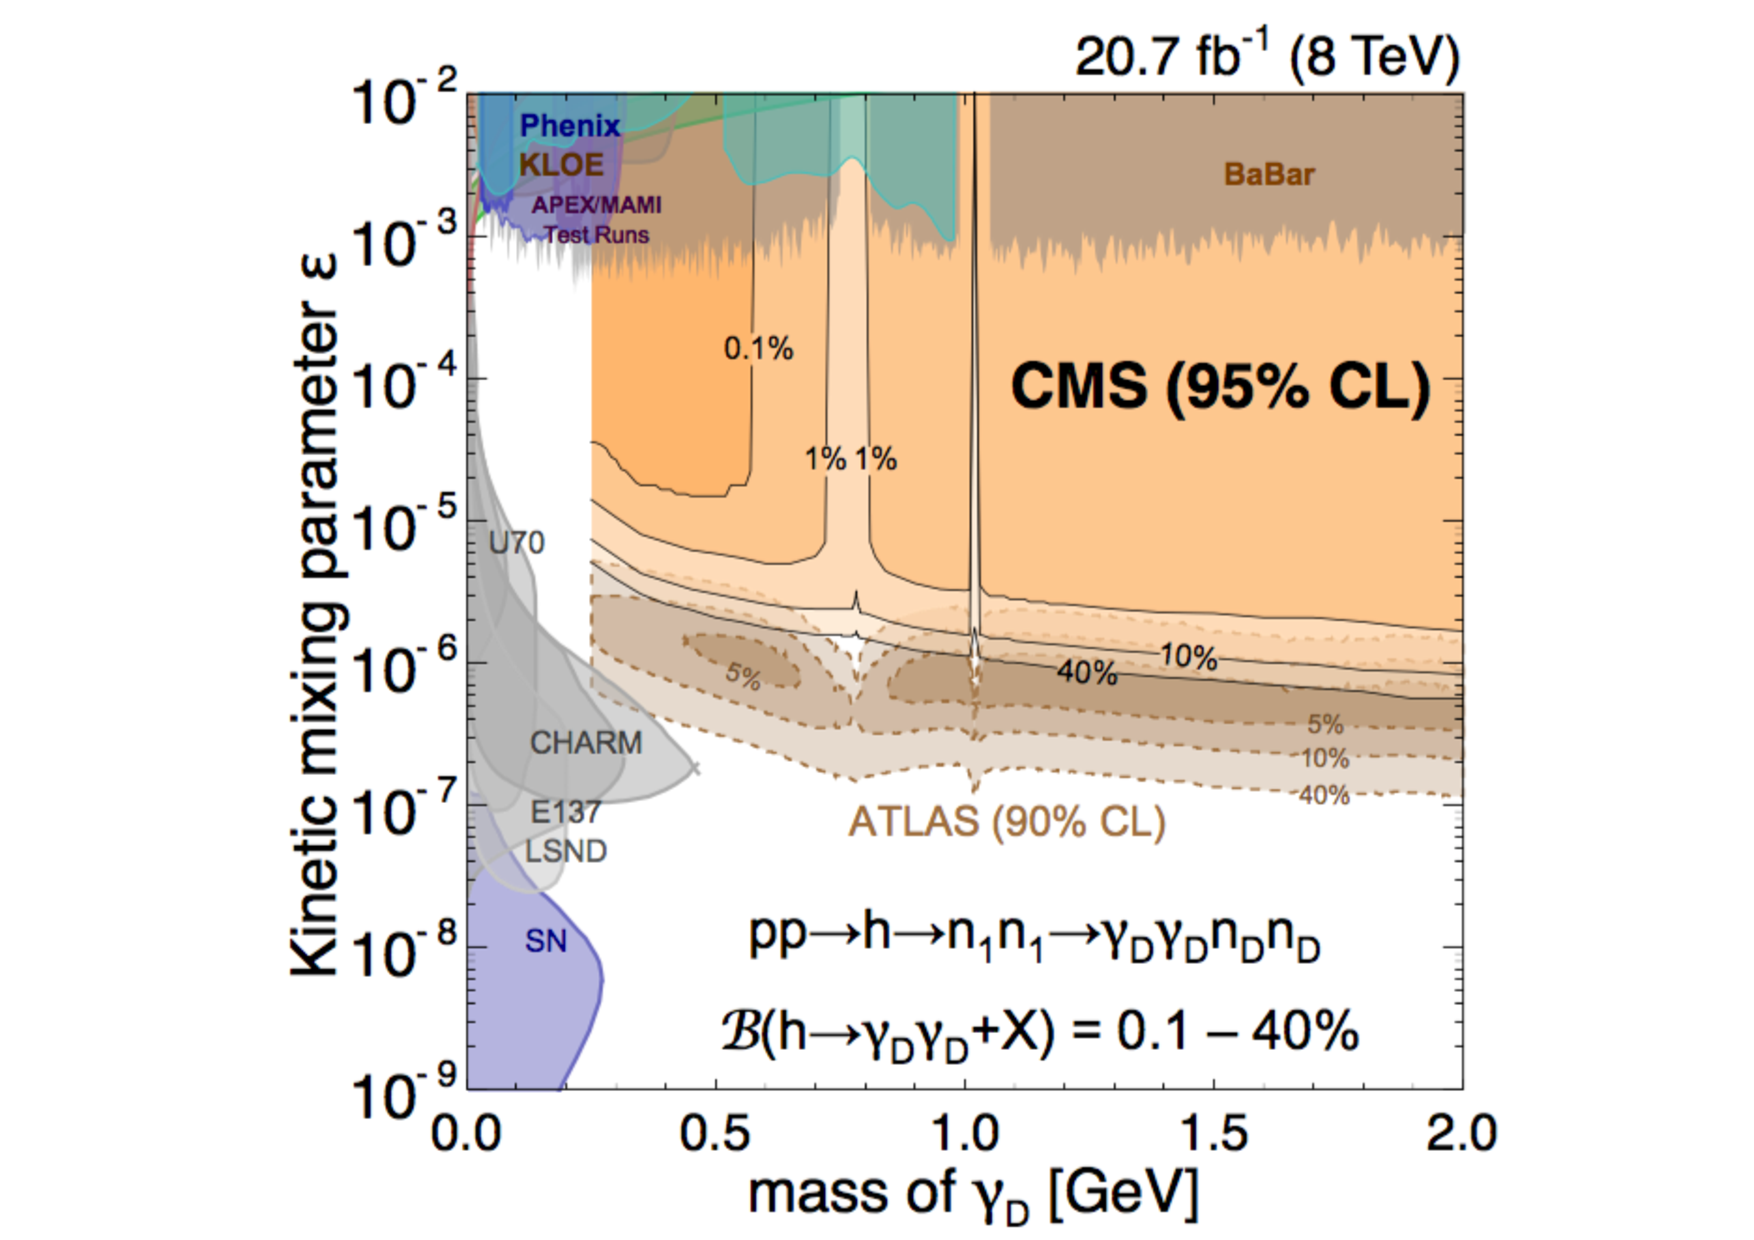
\includegraphics[width=0.7\textwidth]{plots/Limit_Eps_mass_v6.pdf}
\caption{Comparison of the lepton-jet searches at ATLAS~\cite{Aad:2014yea} and CMS~\cite{Khachatryan:2015wka} on the dark photon scenario~\cite{Falkowski:2010cm} vis-a-vis dark photon limits coming from low-energy experiments.}
  \label{fig:dark_photons_CMS_ATLAS}
\end{figure}

LHCb has a search that looks for the direct production of dark photons \cite{Aaij:2017rft}, as opposed to dark photon production in decays of the Higgs. As a result of the direct production, dark photons do not tend to be highly boosted in the transverse direction. Events are required to have a single muon with $p_{\rm T}>1.8$ GeV, or two muons with a product of transverse momenta $\gtrsim(1.5\,\,\mathrm{GeV})^2$. 
For the prompt dark photons search, events are reconstructed at trigger level so that all online reconstructed particles are recorded, while the rest of event information is discarded~\cite{Aaij:2016rxn}.
The displaced search constrains previously uncovered dark photon parameter space around masses of $\sim300$ MeV, while the prompt search constrains entirely new territory above 10 GeV.
 
The LHCb searches for displaced leptons in rare $B$ meson decays~\cite{Aaij:2015tna,Aaij:2016qsm} rely on standard techniques to identify the $B^\pm$ decay vertex and the kaons and pions in the event, and the $m(\mu^+ \mu^-)$  variable is scanned for excesses. The $X \to \mu^+ \mu^-$ vertex is not required to be displaced from the $B^\pm$ vertex, and thus the constraints apply to both prompt and long-lived particles. The analysis probes LLP masses of 214 (250) MeV $< m_X < $ 4350 (4700) MeV for the $B^0 \to K^* \mu^+ \mu^-$ ($B^+ \to K^+ X, X \to \mu^+ \mu^-$) process, with the mass range being limited by kinematics. 

To summarize, the lepton searches rely on fairly standard lepton identification, with vertex reconstruction being performed mostly offline. Searches for leptonically-decaying LLPs typically enjoy low trigger thresholds and good sensitivity to LLP production rates. A major outstanding challenge, however, are LLP decays to $\tau$ leptons, which lie at the interface between hadronic and leptonic searches. Such decays are very well motivated from the theoretical point of view, as a Higgs-like scalar would decay about 300 times more into $\tau^+ \tau^-$ if kinematically allowed, and also one could have large rates into \emph{e.g,} $\tau^+ \mu^-$.   A displaced hadronic $\tau$ is a striking object, and most likely will have few backgrounds. Hence, limits on exclusive displaced $\tau$s would be of upmost importance~\footnote{We note that if the $\tau$ originate from outside the tracker, the hadronically decaying taus are indistinguishable from other displaced hadrons. For instance, in the ATLAS Muon RoI study~\cite{Aad:2015uaa} the results are interpreted for a model with a scalar particle with Higgs-like couplings to SM fermions, which includes a branching fraction into $\tau^+ \tau^-$. However, if the $\tau$ originates from the ID, the low number of tracks associated to it (1-3) will not fulfill the requirements of the ATLAS study to having 5 or more tracks associated to a DV.}.

As the leptonic searches explicitly require opposite-sign leptons, the same-sign lepton signature (motivated from Majorana neutrinos, see the LHCb search in Section \ref{subsec:dsemilep}, or heavy, doubly charged LLPs) is currently neglected.

Lepton-jet searches currently cover only final states with at least two LLPs and some muons in the final state\footnote{The ATLAS 8~TeV search~\cite{Aad:2014yea} included a search channel with two electron-only lepton-jets, but the performance was poor and it was excluded from the final result.}, and the same statement currently applies to both the LHCb searches for dark photons~\cite{Aaij:2016rxn,Aaij:2017rft} 
 and for LLPs produced in $B$-meson decays. It would be beneficial to have additional searches with one lepton-jet or low-mass, leptonically-decaying LLP (which are motivated in hidden sectors and Majorana neutrinos, for example in Refs.~\cite{Izaguirre:2015pga,Izaguirre:2015zva}). In addition, the status of coverage in the intermediate mass-transition region between ``standard" displaced lepton pairs and lepton-jets is unclear, and may potentially harbor a gap.  

 Heavy Neutral Leptons (HNL) are ubiquitious in New Physics models. They constitute an  important physics case that leads to multi-lepton displaced signatures from $W$ decays, with nice prospects at ATLAS and CMS~(see e.g.~ \cite{Izaguirre2015,Nemevsek:2018bbt,Cottin:2018kmq}). While previous searches were not sensitive to this scenario due to either high-$p_T$ requirements or the requirement of two DVs in the same event, the presence of a prompt lepton from the $W$ allows to relax on these in a dedicated analysis (triggering on the prompt lepton was studied recently in~\cite{Cottin:2018kmq}.)~\footnote{Note that the displaced large transverse impact parameter $e$-$\mu$ CMS search~\cite{CMS-PAS-EXO-16-022} fails to cover this scenario due to the aforementioned lepton veto, which kills the tri-lepton signals discussed in Ref.~\cite{Izaguirre2015}. }. 
The identification of two leptons from the vertex is a powerful discriminant against backgrounds from meta-stable particle decays and hadronic interactions in material. This permits a better exploration of the lower HNL mass range ($3-6$~GeV) than in the semi-leptonic channel (see Section~\ref{subsec:dsemilep}) despite the lower branching ratio. It should be noted that the ambition is to probe mixing to all three neutrino flavors, requiring the capability to reconstruct displaced leptons of all flavors, including taus. 

\subsection{Semi-Leptonic decays}
\label{subsec:dsemilep}

As semi-leptonic signatures include aspects of both hadronic and leptonic LLP decays, many of the previously discussed searches can partially cover these cases, and some do so explicitly. For instance, the ATLAS search for electrons and muons accompanied by tracks~\cite{Aad:2015rba}, the inclusive CMS search for DVs~\cite{CMS:2017oor} (there is an specific model interpretation called $B$-lepton addressing precisely this channel), and the large impact parameter $e-\mu$ pair by CMS~\cite{CMS-PAS-EXO-16-022} are all inclusive with respect to other hadrons produced in the LLP decay, provided the leptons are sufficiently isolated~\footnote{Note that the lepton isolation affects most of the semi-leptonic searches.}. In addition, LHCb has dedicated searches for semi-leptonically decaying  LLPs~\cite{Aaij:2016xmb} and semi-leptonic decays of long-lived Majorana neutrinos coming from $B^{-}$ mesons~\cite{Aaij:2014aba}.   The two CMS searches \cite{CMS:2017oor,CMS-PAS-EXO-16-022} need no further explanation for how they cover semi-leptonic LLPs, but we now describe the rest of these searches in some detail.    

The ATLAS search for a vertex with a lepton accompanied by tracks \cite{Aad:2015rba} uses the same trigger as the dilepton vertex search described in Sec.~\ref{subsec:dleptons}. The DV is required to have a lepton as well as at least four additional displaced tracks associated with it, and the invariant mass of the tracks must exceed 10 GeV.  Thus, the search in principle can have sensitivity down to masses $\gtrsim10$ GeV, although the very high $\pT$ threshold for the displaced electron(photon)/muon typically limits sensitivity for low-mass LLPs: the vertex must contain a muon with $\pT > 55$~GeV or an electron with $\pT > 125$~GeV.

The LHCb search for semi-leptonic LLP decays selects events with a muon trigger, then requires a DV offline~\cite{Aaij:2016xmb}. The results are interpreted in terms of four distinctive topologies: single LLP production in association with a new particle, and double LLP pair production either from Higgs decays or via squark pair production.  Material regions are vetoed, leaving heavy flavor produced either directly or from $W/Z$ decays as the dominant background. The signal discrimination is obtained from a multivariate analysis based on the muon $\pT$ and impact parameter, and subsequently the search is optimized based on the LLP reconstructed mass and the muon isolation. This study is sensitive to lifetimes between 1.5 and 30 mm, as can be seen in Figure~\ref{fig:lhcbsemileptonic}. 

\begin{figure}[htb]
\centering
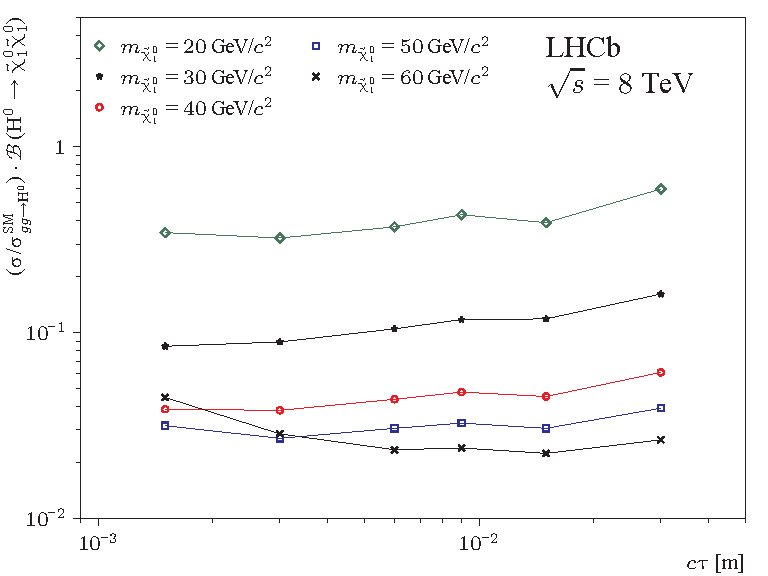
\includegraphics[width=0.9\textwidth]{plots/PAPER-2016-047_sup1.pdf}
\caption{LHCb reach for displaced semi-leptonic decays. Taken from ref~\cite{Aaij:2016xmb}.}
\label{fig:lhcbsemileptonic}
\end{figure}

The LHCb search~\cite{Aaij:2014aba} looks for Majorana neutrinos, $N$, produced in leptonic $B$ decays, $B^\pm\rightarrow \mu^\pm N$, followed by the  decay $N\rightarrow \mu^\pm\pi^\mp$, whether prompt or at a DV\footnote{Some care is required in interpreting the results of the search on a model with a Majorana neutrino, as the original theory interpretation is problematic \cite{Shuve:2016muy}.}. A same-sign muon requirement greatly reduces backgrounds to the search. The sensitivity of the search is limited by the restriction to muons in the final state (so models that predominantly decay to $e$ or $\tau$ are not constrained), as well as the same-sign lepton requirement to only lepton-number-violating processes. More inclusive searches looking for additional $N$ production modes \cite{Gorbunov:2007ak} or searches targeting decays of heavier mesons like $B_c$ \cite{Milanes:2016rzr} could also improve the sensitivity to semi-leptonically decaying LLPs. 

When considering the application of inclusive, hadronic or leptonic searches to semileptonic LLP decays, it is important to understand how the simultaneous presence of leptons and jets in the signal can degrade the sensitivity. For instance, prompt jet searches explicitly veto non-standard jets. Lepton isolation criteria can severely reduce the signal acceptance for a highly-boosted LLP decaying into a lepton and a jet, and they might also veto extra tracks in the events. Thus,  boosted semi-leptonic decays (as might be found in the displaced decay of a low-mass right-handed neutrino produced via $W$ decay) may not be covered by existing searches. 
Another important issue is that the lepton-jet studies express their results in terms of specific dark photon models~\footnote{Recall that the lepton-jet studies also consider the $\gamma_D \to \pi^+ \pi^-$ decay mode.}, which makes it complicated to apply the results to other models. We refer the reader to Sec.~\ref{sec:reint} for a further discussion of this topic.

The signature of HNLs from $W$ decays with displaced semi-leptonic HNL decays is an important item on the search agenda of ATLAS, CMS and LHCb~\cite{Helo2014,Izaguirre2015,Mermod2017,Antusch2017,Nemevsek:2018bbt,Cottin:2018kmq}. The semi-leptonic channel has the highest branching ratio (about 50\% in the relevant mass range~\cite{Gronau1984}) and offers the best discovery prospects at LHC experiments for HNL masses up to 30~GeV as long as a DV mass cut of around 6~GeV is made to mitigate backgrounds from B-mesons, $m_B \sim 5 GeV$. This $6-30$~GeV mass range corresponds to a non-perturbative regime for the hadronisation of the HNL decay products. As the number of charged hadrons significantly affects the DV reconstruction efficiency, the validation of event generator outputs for this process is an important issue currently being addressed by the community (see e.g.~\cite{Cottin:2018kmq}). The ability of LHCb to trigger directly on the HNL decay products and better reconstruct displaced tracks can in some cases compensate for its lower acceptance and luminosity, as exemplified by a recent search for DVs made one muon and several tracks~\cite{LHCb2017,Antusch2017}. This possibly enables LHCb to better probe the more challenging tau channel. Fig.~\ref{fig:HNLsensitivity} shows the overall expected reach of LHC searches in the HNL coupling strength (muon channel) versus mass plane, using assumptions detailed in Ref.~\cite{Mermod2017}, similar to those in Refs.~\cite{Helo2014,Izaguirre2015}. An interesting aspect of the LHC HNL search programme is that backgrounds can be mitigated at high luminosities using the DV feature, making this signature particularly attractive at the HL-LHC. 

The sensitivity of LHC experiments to HNLs is complementary to that of fixed-target experiments which can probe lower couplings thanks to high-intensity beams albeit at lower mass ranges (HNLs from $c$ and $b$ decays). The CERN SPS provides great opportunities with the running NA62 experiment~\cite{NA622017a} and the planned SHiP experiment~\cite{SHiP2015}, which comprise a vacuum decay vessel and spectrometer tracker downstream of the target to reconstruct vertices of long-lived neutral particles~\footnote{The proposed detector FASER would also the capability to reconstruct such vertices~\cite{Kling:2018wct}.}. These are unbeatable for HNL masses up to 2~GeV, where they probe a region of the parameter space favoured in models which explain at once neutrino masses, matter-antimatter asymmetry and dark matter~\cite{Asaka2005b,Canetti2013b,Mermod2017b} (see Fig.~\ref{fig:HNLsensitivity}).

\begin{figure}[t]
\centering
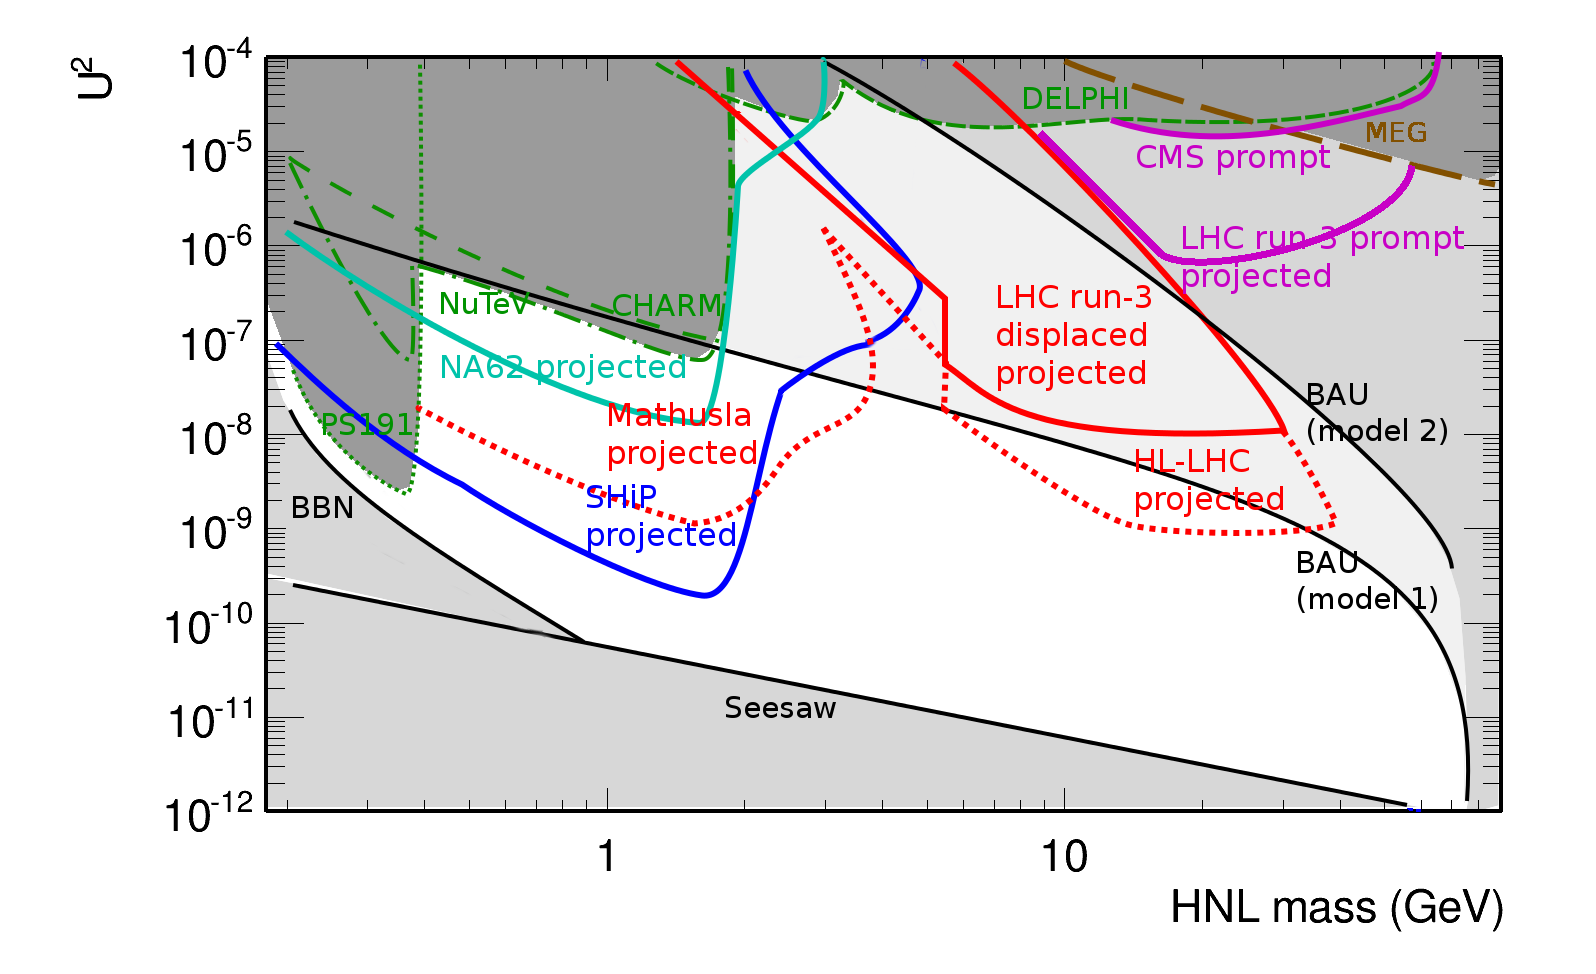
\includegraphics[width=0.99\linewidth]{new_plots/BigPicture.png}
\caption{Summary of projected experimental sensitivities to HNLs in various experiments, in the coupling strength ($U^2$ for dominant mixing to $\nu_\mu$) vs. mass plane. The projections labelled ``LHC run-3'' and ``HL-LHC'' are for HNLs in $W$ decays in general-purpose experiments, and the one labelled ``Mathusla'' assumes the full HL-LHC Mathusla dataset. Prospects at near-future proton beam-dump experiments are also shown for NA62~\cite{Lanfranchi2017} and SHiP~\cite{SHiP2015}. Direct~\cite{Bernardi1988,CHARM1986,NuTeV1999,Delphi1997,CMS2015b} and indirect~\cite{MEG2013,Antusch2015} limits are indicated as dashed green and brown lines respectively. The lines labelled ``Seesaw'' and ``BBN'' show lower theoretical constraints from the observed neutrino masses (normal hierarchy) and primordial nucleosynthesis, respectively~\cite{Canetti2013b}. The lines labelled ``BAU'' are upper theoretical constraints from two different models accounting for baryon asymmetry in the Universe: model 1 requires the lightest HNL to be the dark matter~\cite{Canetti2013b}, while model 2 allows for all three HNLs to participate in leptogenesis~\cite{Canetti2014}. }
\label{fig:HNLsensitivity}
\end{figure}

\subsection{Photonic decays}
\label{subsec:dphotons}

There are two ways in which photons coming from LLP decays do not resemble standard photons. First, they can not be traced back to the PV, thus giving rise to \emph{non-pointing} photons. Second, they can arrive at the electromagnetic calorimeter at a slight different time than expected, referred to as \emph{delayed} photons.  We note that both these kinds of unusual photons can be vetoed when considering prompt photons, and thus the recasting of prompt searches typically provides weaker bounds on LLP scenarios.  ATLAS has a search for non-standard photons~\cite{Aad:2014gfa} using the full 8~TeV dataset, which supersedes the 7~TeV analysis~\cite{Aad:2013oua}, while in CMS there are studies for delayed photons in the ECAL~\cite{CMS:2015sjc} and for non-pointing photons detected via their conversion to $e^+ e^-$ pairs~\cite{CMS:2015gga}. The underlying topology in all these models is the neutralino decay into a gravitino and a photon ($\chi^0_1 \to \gamma \tilde{G}$), ubiquitous in gauge-mediated supersymmetry breaking (GMSB) scenarios~\cite{Dine:1994vc,Giudice:1998bp}. Hence all these studies require to have large $\metm$ in the final state.

The ATLAS study benefits from the capability of the liquid-argon electromagnetic calorimeters to measure the flight direction and the time-of-flight of photons. Resolutions on $\Delta z_\gamma$, the separation between the PV of the event and the extrapolated origin of the photon, and $|\Delta t_\gamma|$, difference of the arrival time of the photon with respect to the prompt case, are as low as 15~mm and 0.25~ns, respectively. The trigger demands two photons within $|\eta| < 2.5$, with transverse energies $E_T$ of 35 and 25 GeV.  
In addition, to guarantee the event comes from a proton--proton collision, a PV with 5 or more tracks with $\pT > 0.4$ GeV is requested.
The offline selection requires two photons with $E_T >$ 50 GeV and $|\eta| < 2.3$, not in the barrel-endcap transition region ($1.37 < |\eta| < 1.52$), at least one of them in the barrel ($|\eta| < 1.37$) and with less than 4 GeV energy deposit in the calorimeter in a cone of $\Delta R =0.4$ around them (\emph{isolation}). In addition, the events are binned in $\metm:$ the $\metm < 20$ GeV bin contains the prompt backgrounds, the 25 GeV $< \metm < 75$ GeV bin is used as the control region, and finally the signal analysis is performed in the $\metm > 75$ GeV bin. This study covers lifetimes from 0.25 to 100~ns in the GMSB framework, the lower limit being a hard cut-off imposed experimentally, as the similarity between background and signal samples in that region makes discrimination rather difficult. The excluded signal rates in this range of lifetimes vary between 0.8 and 150 fb, with the best-constrained value obtained for $\tau \sim$ 2 ns.
 
The CMS study of delayed photons~\cite{CMS:2015sjc} follows a similar approach to ATLAS. The main difference is that it demands only one photon with $\pT > 80$ GeV, but in addition two jets are required. Furthermore, in addition to \met, the vector sum of \met and $E_T^\gamma$, which is denoted $E_{T~{\rm no }\gamma}^{\rm miss}$, is used for background discrimination. (Non)-collisional backgrounds have small (large) \met and  large (small) $E_{T~{\rm no }\gamma}^{\rm miss}$, while for the signal events both variables are large, hence they are both requested to be larger than 60 GeV. The time resolution is 0.372~ns, slightly worse than in the optimal scenario of the ATLAS search. Their reach in lifetimes lies in the 2--30~ns range, excluding signal rates of 10--30 fb.
 
The CMS study of non-pointing photons~\cite{CMS:2015gga} relies on conversion to $e^+ e^-$ pairs. It requires two photons, two additional jets, and $\metm > 60$ GeV. The photon trajectory is obtained from the conversion vertex as the line segment along the momenta of the $e^+ e^-$ track pair, and the impact parameter, $|d_{XY}|$, is defined as the closest distance between the photon and the beam axis, can be determined within approximately 1 mm.
A comparison of the reach of these 8 TeV studies, as well as those using the 7 TeV dataset, can be found in Fig.~\ref{fig:gaga}.
 
%%%%%%%%%%%%%%%%%%%%%%%%%%%%%%%%%%%%%%%%%%%%%%%%
\begin{figure}[htb]
\centering
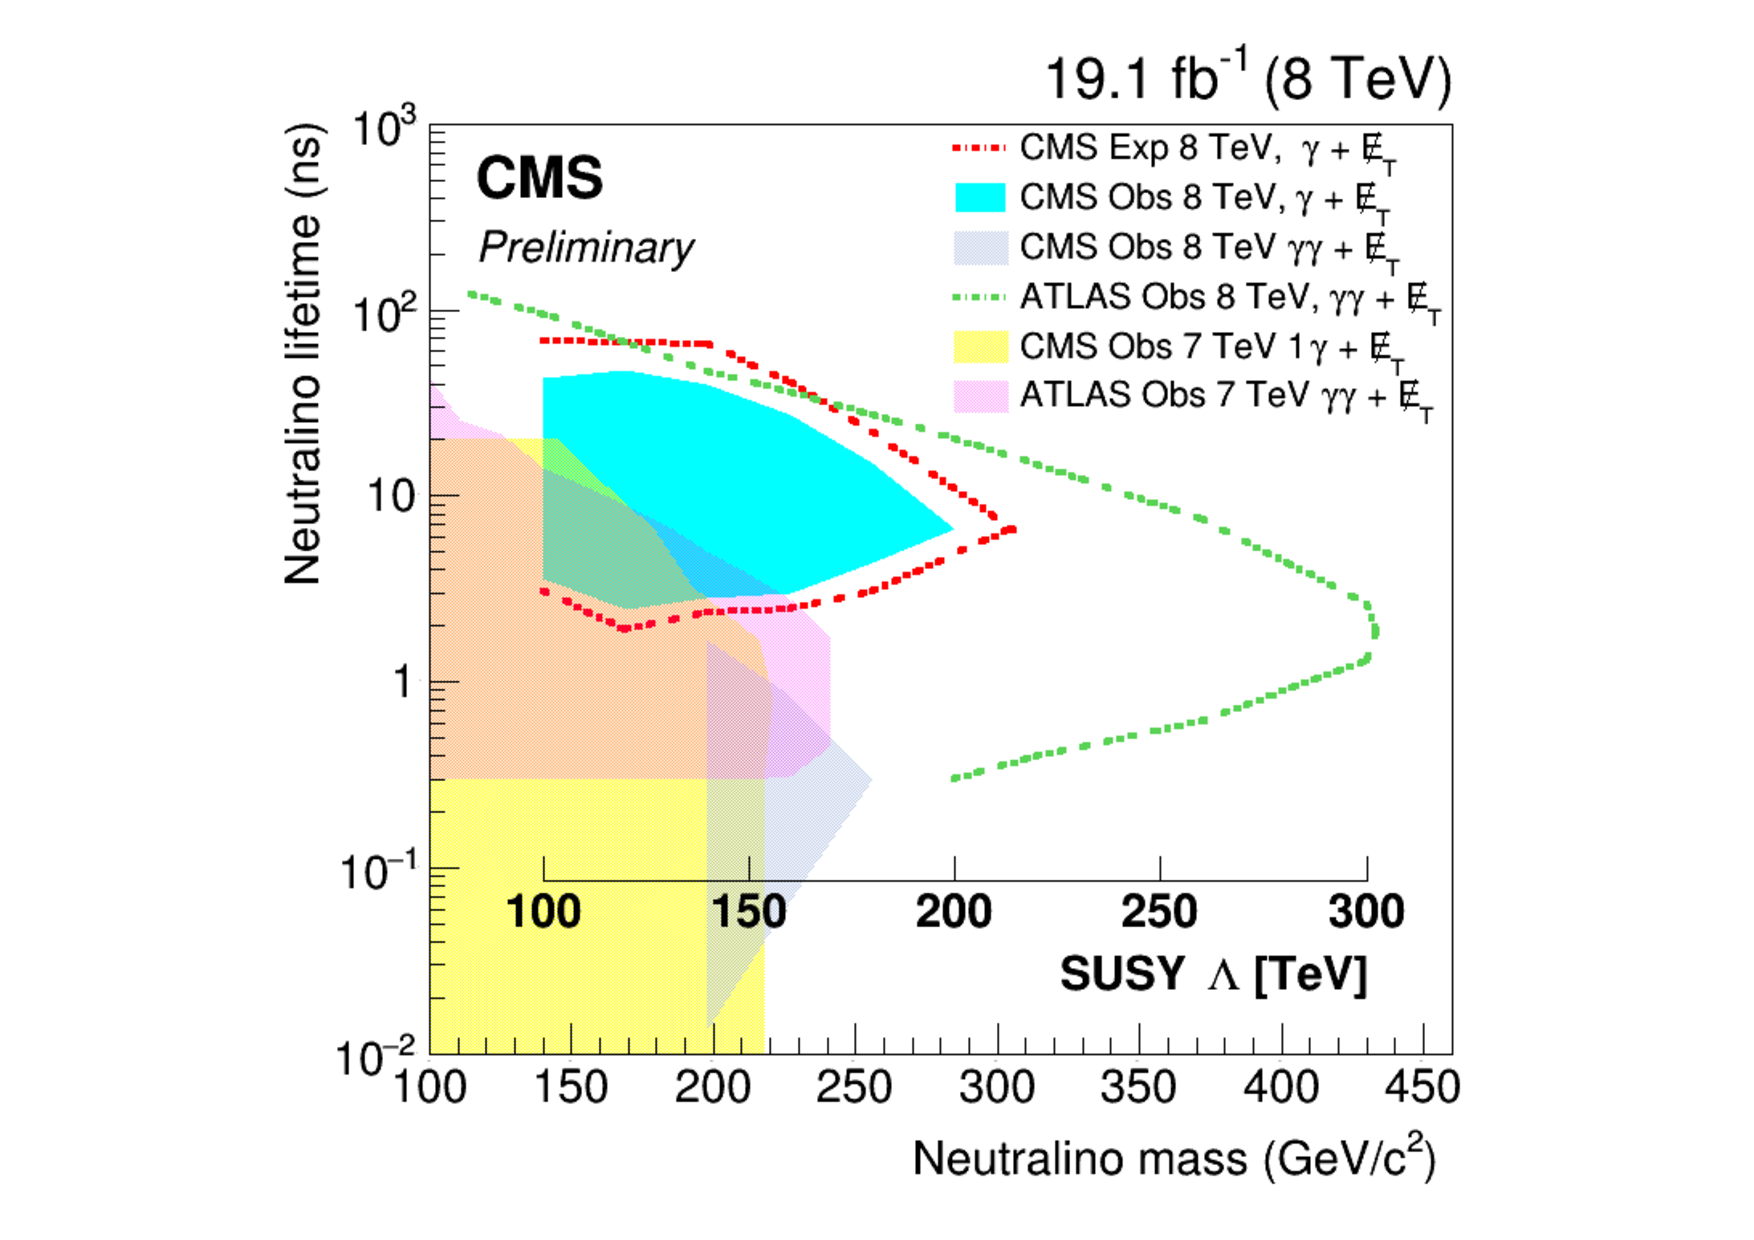
\includegraphics[width=0.7\textwidth]{plots/CMS-PAS-EXO-12-035_Figure_016-a.pdf}
\caption{Summary of the $\gamma + \metm$ searches from ATLAS and CMS, displayed assuming the same GMSB model. Taken from reference~\cite{CMS:2015sjc}. 
}
  \label{fig:gaga}
\end{figure}
%%%%%%%%%%%%%%%%%%%%%%%%%%%%%%%%%%%%%%%%%%%%%%%
 
The gaps in these studies are straightforward to identify. The requirement of large $\metm$ is due to the fact that all of these studies have an underlying theoretical picture of neutralinos decaying into gravitinos and photons, motivated from GMSB scenarios.   Hence, these searches do not cover cases without the presence of missing energy, including LLPs that decay to $\gamma \gamma$, $l \gamma$ or $j \gamma$, although either mis-measurement of jets or the photon decay geometry could fake large missing energy to provide moderate constraints. With the exception of the CMS study~\cite{CMS:2015sjc} which requires two additional hard jets, all of these analyses require two displaced photons.  A single displaced photon signature can occur in motivated models:~it can easily arise, for example, from a very slightly mixed electroweak triplet and singletm belonging to the SUSY Simplified Model category from Sec.~\ref{sec:simplifiedmodel}. Furthermore, as discussed in section~\ref{subsec:djets}, a single LLP in the detector can also arise for very large lifetimes of neutral LLPs, which limits the reach at longer lifetimes.

\subsection{Other exotic long-lived signatures}
\label{subsec:funnytracks}

In this section we present the analyses that are based on exploiting properties of other exotic long-lived signatures, such as non-standard tracks.  We summarize in detail the existing searches for heavy stable charged particles (HSCP), disappearing tracks (DT), stopped particles (SP) and monopoles, and describe  existing ideas on how to look for quirks and SIMPs (Strongly Interacting Massive Particles).

\subsubsection{Heavy Stable Charged Particles (HSCP)} 
\label{subsec:ExpHSCP}

The search for HSCPs at CMS~\cite{Chatrchyan:2013oca,CMS:2016ybj} and ATLAS~\cite{ATLAS:2014fka,Aaboud:2016uth} rely on two key properties. First, particles that are massive and/or electrically charged with $Q \ne \pm e$ have a  characteristic ionization energy loss ($dE/dx$) distinctively different than SM particles. 
%This property can be measured in the tracker.
Second, HSCPs are typically heavy and move with a speed smaller than the speed of light, $\beta = v/c < 1$. Thus, compared to a particle with $\beta \approx 1$, they require a longer time-of-flight (TOF) to reach the outermost components of the detector (calorimeters and muon chambers).  Interactions of the HSCP with the material in the detector can change the electric charge of the HSCP and they occur randomly. Hence both CMS and ATLAS perform separate \emph{tracker-only} and \emph{tracker + TOF} studies in the language of CMS~\footnote{ATLAS measures $\beta \gamma$ from $dE/dX$ and $\beta$ from time-of-flight and extracts an independent mass, $m_{\beta}$ and $m_{\beta \gamma}$, from each measurement.}. The event selection relies on standard single-muon or large-missing-energy triggers. The offline selection relies on identifying the signal events from quality requirements on the tracks using discriminator variables built from track observables. 

The theoretical interpretation of a signal or limit depends on whether the HSCP carries both color and electroweak charges. If it carries a color charge, the default benchmarks correspond to $R$-hadrons, namely HSCPs that hadronize with SM particles via the strong force (e.g gluino--gluon, quark--squark states). In the absence of a color charge, the signal is exemplified by long-lived sleptons in the context of gauge-mediated and anomaly-mediated SUSY breaking. Both ATLAS~\cite{ATLAS:2014fka} and CMS~\cite{CMS:2016ybj} studies employ these two scenarios\footnote{The ATLAS R-hadron searches using the 13 TeV dataset have recently been presented in reference~\cite{Aaboud:2016uth}. }.
Finally, CMS also looks for HSCPs coupling only to hypercharge (and hence possessing only couplings to $\gamma$ and Z), while ATLAS has a search inspired by electroweakinos in SUSY:~it considers the associated production of a neutral and an electrically charged LLP (chargino--neutralino), and thus only one HSCP plus missing energy are required.

The HSCP search conducted by LHCb~\cite{Aaij:2015ica} is slightly different.
Instead of exploiting $dE/dx$ and time-of-flight, they use the lack of radiation in the ring imaging Cherenkov detector (RICH). Events are required to pass a high-\pT single-muon trigger ($\pT(\mu) > 15$ GeV). Two opposite sign muons are then required, each with \pT above 50 GeV and an invariant di-muon mass above 100 GeV, to suppress muons coming from Drell-Yan production, the main background for this search. In addition, particles must have $\beta > 0.8$, set by the efficiency of the muon chambers to reconstruct slow particles. As electrons and hadrons interact more with the calorimeter than an HSCP, a deposit in the calorimeter of less than 1\% of the momentum of the particle is required.  The results are interpreted in the context of stau pair production.

To summarize, these searches are robust, but the trigger efficiency drops with decreasing $\beta$. It would be worth exploring trigger strategies to probe such values of $\beta \lesssim 0.6 - - 0.8$.
%$\beta \lesssim 0.6 - - 0.8$.
%present no obvious weak points. Standard triggers and tracking algorithms are used, and the analysis methods are well-understood and have been extensively validated against data. While the HSCP strategies are robust, 
%we encourage the experimental collaborations to continue pursuing improvements for these searches. In particular it would be worth exploring ideas to probe particles with $\beta < 0.8$, which at the moment is an inherent hardware limitation. 
The small number of signal events that would be produced for HSCPs above current limits render the sensitivity highly dependent on the understanding of the background and the control of the systematics.

\subsubsection{Disappearing tracks (DT)} 

Massive charged particles traveling in the detector can decay to a lighter, almost mass degenerate neutral state, emitting a SM charged particle (typically a pion or a muon). While at first glance a small mass gap na\"ively seems like a hallmark of tuning, near degeneracies often occur naturally as a result of a symmetry. In fact, electroweak symmetry generically leads to small mass splittings $\Delta$ between components of a single electroweak multiplet. For example, ${\cal O} (100 $ MeV) splittings arise between the different components of an electroweak multiplet~\cite{Thomas:1998wy,Cirelli:2005uq} due to EW gauge boson loops~\footnote{For a single fermionic multiplet, the splitting can only be altered by higher-dimensional operators, and thus it is harder to vary $\Delta $ from the 1-loop EW value. For other cases, such as mixing with additional particles, the actual splitting can differ greatly than this 1-loop EW value.}. If the SM particle is sufficiently soft it can not be reconstructed, and then a charged track seems to vanish: this is thus referred to as a disappearing track~\footnote{If the charged particle could be reconstructed this case is often referred to as \emph{kinked track}.  However, as the kinked portion has a very large impact parameter, without a serious attempt to capture the kink these tracks too simply disappear.}.  The actual lifetime of the charged particle is highly sensitive to the precise value of the mass splitting. For instance, the well studied cases of a fermionic doublet with $Y=1/2$ and a fermionic triplet with $Y=0$, reminiscent of a Higgsino and Wino in supersymmetry, respectively, have mass splittings of $\Delta = 355$ and 166 MeV up to small corrections, but the corresponding $c \tau$ differ by almost an order of magnitude: 6.6 mm versus  5.5 cm\footnote{While these values set a concrete physics target, we stress again that the mass splitting can be arbitrary in other corners of the BSM parameter space (even within SUSY). For instance,  $\tilde{\tau} \to \tau \tilde{\nu}$ (where the stau and sneutrino masses are free independent parameters) or for scalar particles (e.g: $H^+ \to \mu^+ H^0$), where the mass splitting and the overall mass scalar are set by arbitrary quartic couplings.}. This is because the lifetime, $c\tau$, depends on the third power of the mass splitting in these scenarios \cite{Thomas:1998wy,Cirelli:2005uq}. 

Before 2017, both ATLAS~\cite{Aad:2013yna} and CMS~\cite{CMS:2014gxa} required a track to travel about 30 cm in order to be reconstructed, giving good coverage of the Wino scenario. These 30 cm correspond to four hits at ATLAS, three in the pixel layers plus one in the silicon tracker, and to seven hits in the pixel and trackers of CMS. The search uses a trigger requiring an ISR jet against which the charged particle recoils, along with the presence of large missing energy. The disappearing track is reconstructed offline and needs to fulfil a few quality criteria (isolation, \pT threshold, etc). A phenomenological study~\cite{Mahbubani:2017gjh} had shown that reducing the distance from 30 to 10 cm would give coverage to the elusive Higgsino scenario, moving the expected reach up to 400 GeV, trumping over the expected mono-jet reach of 250 GeV~\cite{Schwaller:2013baa,Low:2014cba,Barducci:2015ffa}. Later ATLAS presented a study~\cite{ATLAS-CONF-2017-017} using 13 TeV data and exploiting the presence of a new innermost pixel layer (IBL). This addition allows for all four hits to be in the pixel, with the outermost pixel layer now at 12.25 cm,  granting sensitivity to lower values of $c \tau$. The summary for disappearing tracks at ATLAS for the Wino case can be seen in the left panel of Figure~\ref{fig:ewkinosearches}, while in the right panel we show the constraints for Higgsinos from reference~\cite{Mahbubani:2017gjh}.

\begin{figure}[htb]
\centering
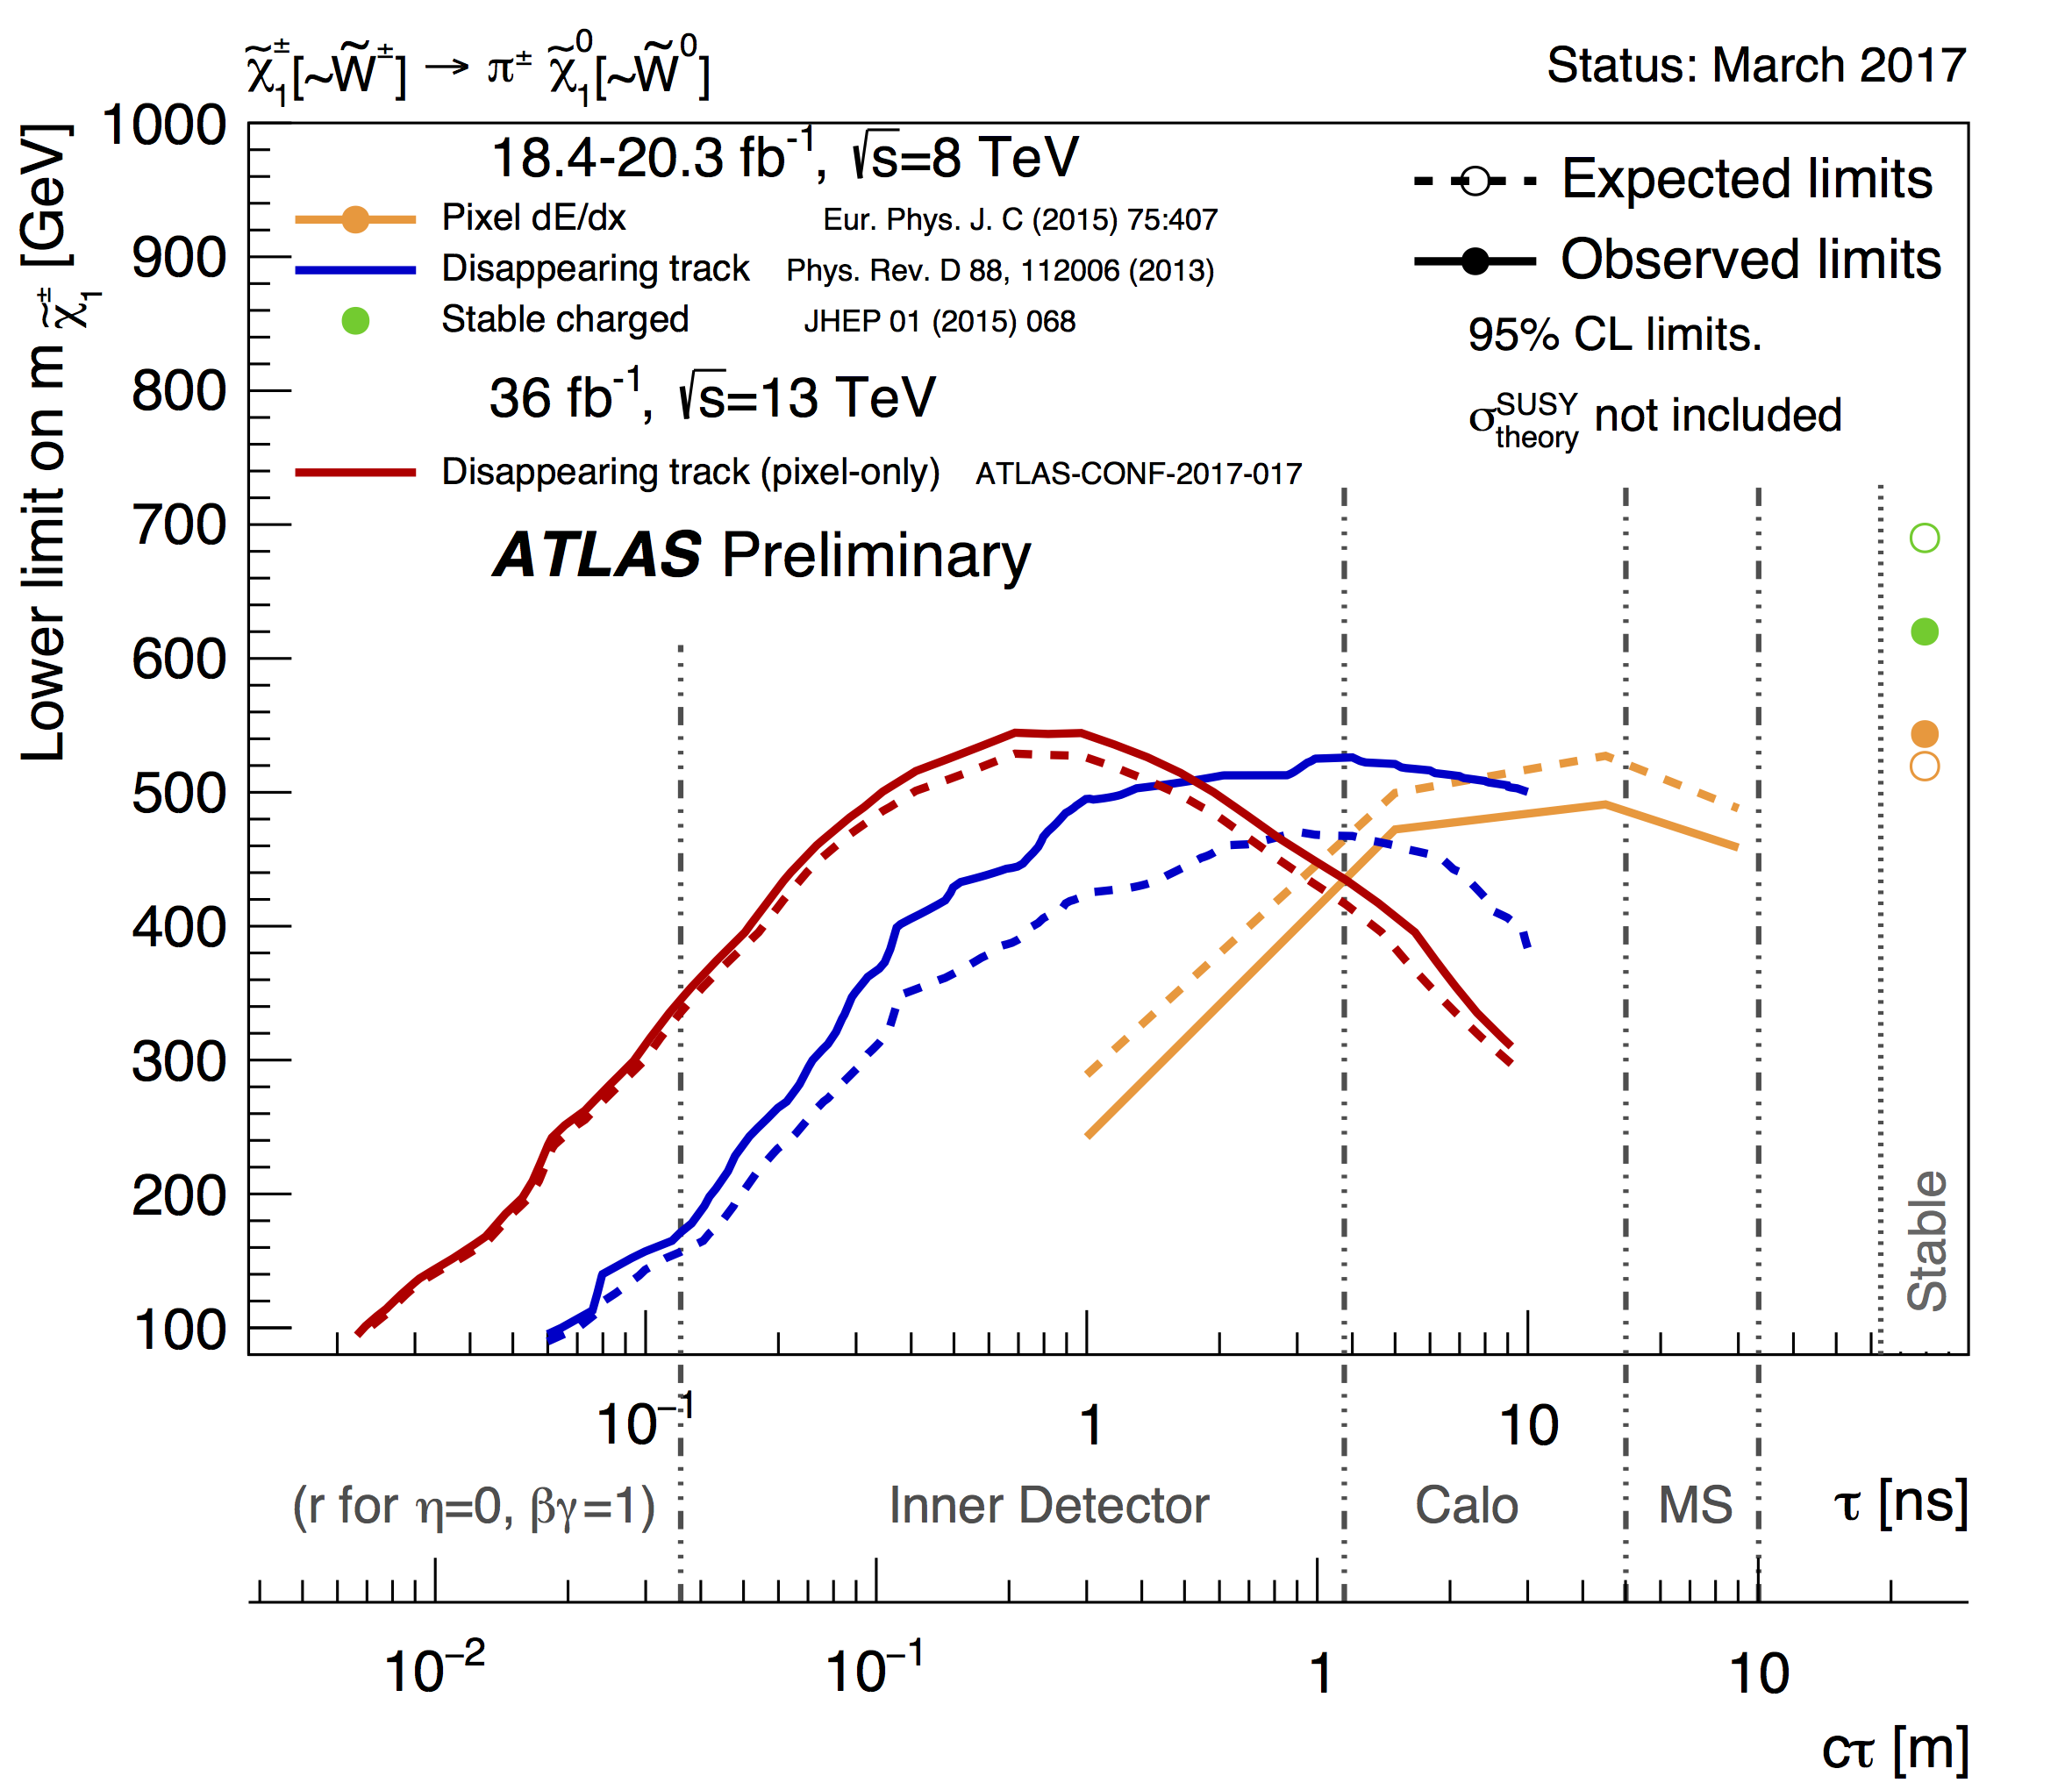
\includegraphics[width=0.44\textwidth]{plots/ATLAS_SUSY_LLPChargino.png}
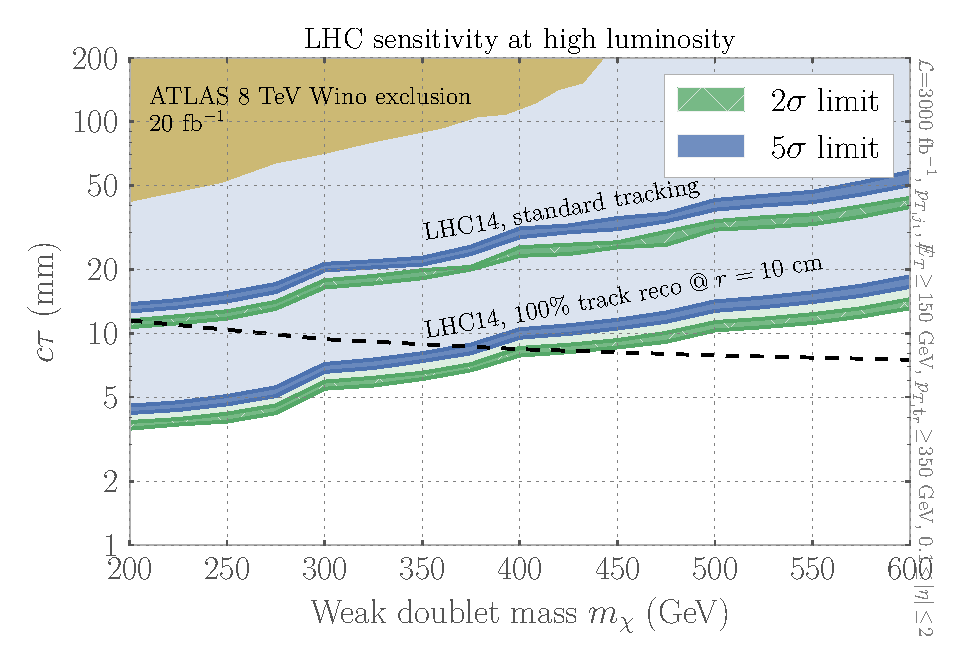
\includegraphics[width=0.54\textwidth]{plots/Higgsino_Significance14}
\caption{Summary of the status of Wino searches in ATLAS (left panel) and HL-LHC expected constraints on the Higgsino scenario (right). Taken from~\cite{ATLAS:summary} and ~\cite{Mahbubani:2017gjh} respectively.}
  \label{fig:ewkinosearches}
\end{figure}

At LHCb the prospects for a disappearing track analysis with the present detector are poor. Currently, the momentum of the track can only be measured if the particle passes through the Tracker Turicensis (TT), which is about 3~m away from the IP. Particles decaying in the VELO or RICH1 system will not leave a fully-measurable track and will be swamped in a background of SM processes such as kaon decays, which would give a similar signature in the detector components before the magnet. Detector improvements such as additional magnets, better particle identification (PID) at low momentum and additional layers might lead to some sensitivity for ${\cal O}$(cm) lived tracks.

%If the detector were improved (by e.g: adding station magnets, better PID at \textcolor{red}{To be completed.}

To summarize, the searches for disappearing tracks present a few drawbacks. Using an ISR-jet trigger means a price is paid in terms of signal sensitivity: reference~\cite{Mahbubani:2017gjh} has shown that significantly lowering the \pT threshold of the jet (or directly triggering on the momentum of the disappearing track~\footnote{While currently there are some proposals to trigger on tracks~\cite{Gershtein:2017workshop}, those only apply to standard tracks. In particular, the new fast track reconstruction (FTK) system at ATLAS requires more than 10 hits~\cite{Holmes:2017workshop,Horyn:2017workshop,Ilic:2017sdh} }) would lead to a factor of 2 increase in the number of signal events. It is also clear that better access to lower lifetimes is needed; thus, adding new layers as close as possible to the beampipe (and/or having double layers instead of single ones) is a desirable feature.

\subsubsection{Stopped particles (SP)} 

If an HSCP is produced with very low kinetic energy, it can come to rest in the detector due to interactions with the detector materials. This most likely occurs in the calorimeters (due to their high density) or in the muon chambers. The HSCP can then decay at a later time when no collision is taking place (an out-of-time decay). This experimental restriction severely restricts the background processes, with the dominant backgrounds coming from cosmic rays, beam halo and instrumental noise.

In the Run-I analyses from ATLAS~\cite{Aad:2013gva} and CMS~\cite{Khachatryan:2015jha},  events are selected with a dedicated trigger selecting  bunch crossings which are empty and have no bunches of protons nearby. The analyses require a jet with \pT ($E$) above 30 (50) GeV at ATLAS (CMS). ATLAS further supplements the hardware trigger by requiring $\pT(j) > 50$ GeV, $|\eta| < 1.3$ and $E_T^{\rm miss} > 50$ GeV, rejecting instrumental noise. In addition, CMS has a search that triggers on out-of-time muons~\cite{Sirunyan:2017sbs} using the 13 TeV dataset. The latter also employs the displaced stand-alone (DSA) muon reconstruction algorithm~\cite{CMS-DP-2015-015}.

An offline selection procedure follows aimed at reducing the main backgrounds. Since, as mentioned, the particles are most likely stopped in the calorimeters or muon chambers, the information coming from the muon chambers is crucial to identify the signal events. 
Muons coming from cosmic rays can be identified due to their distinctive topology. Beam halo is the result of protons interacting with residual gas in the beampipe, the beampipe itself, or collimators upstream from the interaction point. Most particles will not travel far before being absorbed by various structures, but muons will travel parallel to the beam and can leave calorimeter deposits out of time with a proton--proton collision. 
However, these deposits will often present with corresponding horizontal tracks in the muon systems and can thus be efficiently vetoed. Instrumental noise is rejected in CMS by exploiting the anomalous response in the HCAL. 

Searches for charged particles crossing the detector (HSCP searches for short) are typically much more sensitive to any signature that can have a charge, so stopped particle searches are not expected to be a discovery mode for most simple new physics scenarios with charged LLPs. However, in case of a positive signal, HSCP searches might not provide much information. In such a case, SP searches allow to properly study the decays of the newly discovered LLP. 
Moving forward, as luminosity rises and the number of empty bunch crossings per fill decreases it might be worth considering how higher energy and triggering thresholds could control backgrounds and allow for access to novel physics decaying off-time from the rest of the event. 

\subsubsection{Magnetic Monopoles} 

ATLAS~\cite{Aad:2015kta} has a dedicated search for highly ionizing particles (HIPs), which encompass a variety of new physics scenarios, such as magnetic monopoles, dyons (particles with both magnetic and electric charge), stable microscopic black holes, etc. For the sake of concreteness, we focus on magnetic monopoles but the interpretation in terms of other models is straightforward.

The main phenomenological feature is that magnetic charge is quantized in units of $g_D = 2\pi/e \approx 68.5$. Hence, a magnetic monopole behaves as a particle with at least 68.5 electron charges, leading to an unusually large ionization power in matter, so that they would quickly stop in the detector as HIPs lose energy at spectacular rates. Because of the large QED coupling of magnetic monopoles, a perturbative calculation of the cross section is invalid and there is no accurate determination of the production rate, but a na\"ive Drell-Yan production cross section is provided for the purposes of comparison. The specifics of the detector restrict the sensitivity of this search to magnetic charges $g < 2 g_D$ because a large fraction of the monopoles stops in the material upstream of the electromagnetic calorimeter, as the latter is used for the L1 trigger~\cite{DeRoeck:2011aa}.
We note that larger magnetic charges can be tested by the MoEDAL experiment~\cite{MoEDAL:2016jlb}, which is described in detail in section 5.

ATLAS~\cite{Aad:2015kta}  has a dedicated trigger for HIPs based on identifying relevant RoIs in the ECAL and subsequently counting the number of hits in the TRT. As well, the fraction of TRT hits that are high-threshold (HT), meaning that they have an ionization larger than $\sim3$ times that expected from a SM particle, is used as a discriminant. The analysis selects events based on the fraction of TRT-HT hits within a track matched to an EM cluster deposit, and how the energy deposits are distributed in the different layers of the ECAL. It is important to note that due to the lack of a consistent theory, the signal simulation is performed by re-scaling Drell-Yan production at leading order and assuming no coupling to the Z-boson. The HIPs are assumed to have either spin-0 or 1/2. The spin does not affect the interaction with the material, but the angular distributions are different according to angular momentum conservation; however, there is anyways no perturbative theoretical prediction for the angular distribution. Cross-section limits for $0.5 < |g|/g_D < 2$ are set for masses in the $890--1050$ ($1180--1340$) GeV for the spin-0 (1/2) case.

The coverage in LHC Run-2 of magnetic monopoles in the $g_D-\sigma$ plane is displayed in fig~\ref{fig:magnetic_monopole_reach}.
\begin{figure}[htb]
\centering
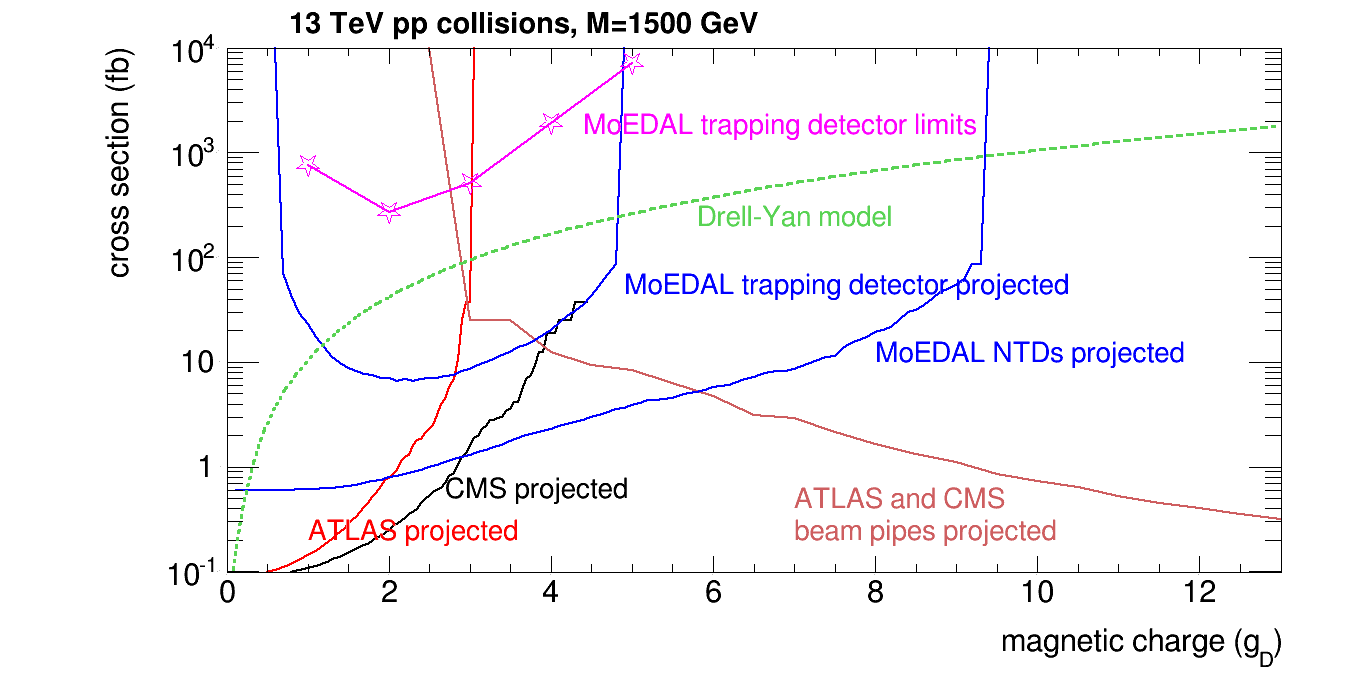
\includegraphics[width=0.8\textwidth]{plots/monopoles_xsec_13TeV_3events}
\caption{Comparison of the MoEDAL, ATLAS and CMS reach for magnetic monopoles. The curves assume 3 signal events and a total integrated luminosity of 50 fb$^{-1}$ for 13 TeV collisions. Source: private communication from P. Mermod, updated version of existing FIg. in~\cite{DeRoeck:2011aa}.}
\label{fig:magnetic_monopole_reach}
\end{figure}

\subsubsection{Quirks}

Quirks are particles charged under both the SM and a new confining gauge group \cite{Kang:2008ea}, referred to here as ``infracolor'' (IC). The defining property of quirks is that the tree-level quirk masses $m_Q$ are above the confinement scale $\Lambda_{IC}$ (this is like QCD but with no light-flavored quarks), so that there is never enough local energy density to pop new quirks out of the vacuum.  A pair of a quirk and an anti-quirk can live in a quantum mechanical bound state that can separate by macroscopic distances $\ell \sim \frac{m_Q}{\Lambda_{IC}^2}$, remaining connected by an infracolor flux tube. The infracolor flux tube exerts a tension on each quirk that causes its trajectory to differ from the expected helicoidal ones for SM particles. Although well-motivated by hidden-valley models \cite{Strassler:2006im}, we stress that quirks are not exclusive to hidden valleys, contrary to popular lore.

The collider phenomenology depends greatly on the size of $\ell$.  If $\ell$ is below the mm scale, the individual quirks are not distinguished from one another and the anomalous track can not be seen. However, the pair (which is overall neutral, and therefore does not bend in the tracker magnetic field) appears as a single highly ionizing straight track with missing energy aligned with it, the latter arising from miss-measuring the track momenta.
The D0 collaboration has searched for precisely this signature \cite{Abazov:2010yb}, requesting an additional jet for trigger purposes, finding lower bounds on quirk masses of 107, 119 and 133 GeV for SU(2), SU(3) and SU(5) gauge groups. However, no extensions of this search to higher mass have been performed at the LHC, and the existing HSCP searches require a fractional certainty on the tracks momenta that a straight track cannot provide.

Conversely, if $\ell$ is very large then the existence of the confining force has no effect on the quirk motions, and HSCP searches  apply directly to the quirk case, with quirks charged under QCD yielding $R$-hadrons and uncolored quirks leading to slepton-like signatures. We refer the reader to the HSCP section for more information.

For intermediate values of $\ell$, there are interesting phenomenological prospects at the LHC that have been recently studied theoretically~\cite{Farina:2017cts,Knapen:2017kly}, but for which there are no current public searches by the LHC collaborations. The first study~\cite{Farina:2017cts} has recasted mono-jet~\cite{CMS:2016pod,Aaboud:2016tnv} and HSCP searches, finding bounds up to 1.7 TeV for colored-quirk masses. In addition, it has also proposed using the CMS dataset taken with zero magnetic field. In this dataset, all SM particles are expected to follow a straight trajectory, but the quirks would still bend due to the string tension. The second study~\cite{Knapen:2017kly} has proposed a new algorithm to search for quirks, exploiting the fact that the quirk and anti-quirk pair should lie in the same plane with the highest sensitivity in the $\ell \sim 1-10$ mm range. This allows to avoid fitting the non-helicoidal trajectories, and has the potential to extend the sensitivity to quirks well beyond the current mono-jet and HSCP limits.

Because of the non-standard nature of the tracks, quirk phenomenology poses substantial challenges in their experimental reconstructions, and the lack of constraints on quirks have already attracted the attention of the ATLAS, CMS and LHCb experiments. It would be desirable to test how the phenomenological proposals in Refs.~\cite{Farina:2017cts,Knapen:2017kly} can perform in a realistic detector simulation of one of the LHC experiments.

\subsubsection{Strongly interacting massive particles (SIMPs)}

Strongly interacting massive particles (SIMPs) can be motivated by astrophysical observations of dark matter that do not fully agree with the WIMP paradigm (missing satellites, core-vs-cusp problem see e.g.~\cite{2010arXiv1009.4505B,2011MNRAS.415L..40B,Weinberg:2013aya,1742-6596-437-1-012001}). These particles are assumed to interact strongly with baryons. Consequently, the experimental signature is little to no signal in the tracker and the ECAL, and large energy deposits in the HCAL. Such a final state with trackless jets also arises in the context of emerging jets~\cite{Schwaller:2015gea}, and ATLAS has a trigger for trackless jets in association with a soft muon (where the muon is required to exit level 1 of the trigger)~\cite{ATLASLLPTriggers}. Additionally, the CalRatio trigger and associated search for displaced hadronic decays (addressed in Section~\ref{subsec:djets}) presents with a similar signature and could provide some coverage of this signature.  

An LHC phenomenological study of SIMPs was carried out in Ref.~\cite{Daci:2015hca}. We summarize the main points of the study here. In their setup, SIMPs interact with the SM via an attractive potential (either scalar or vector mediator) coupling SIMP pairs with $q\bar{q}$ pairs. The proposed analysis selects events with high \pT back-to-back jets within the tracker, exploiting the charged energy fraction within a jet to discriminate signal from background.  The astrophysical experimental constraints on this scenario are compared with the expected reach of this search and that of monojets in figure~\ref{fig:simps}. Currently there is an ongoing analysis in CMS pursuing this strategy.

\begin{figure}[htb]
\centering
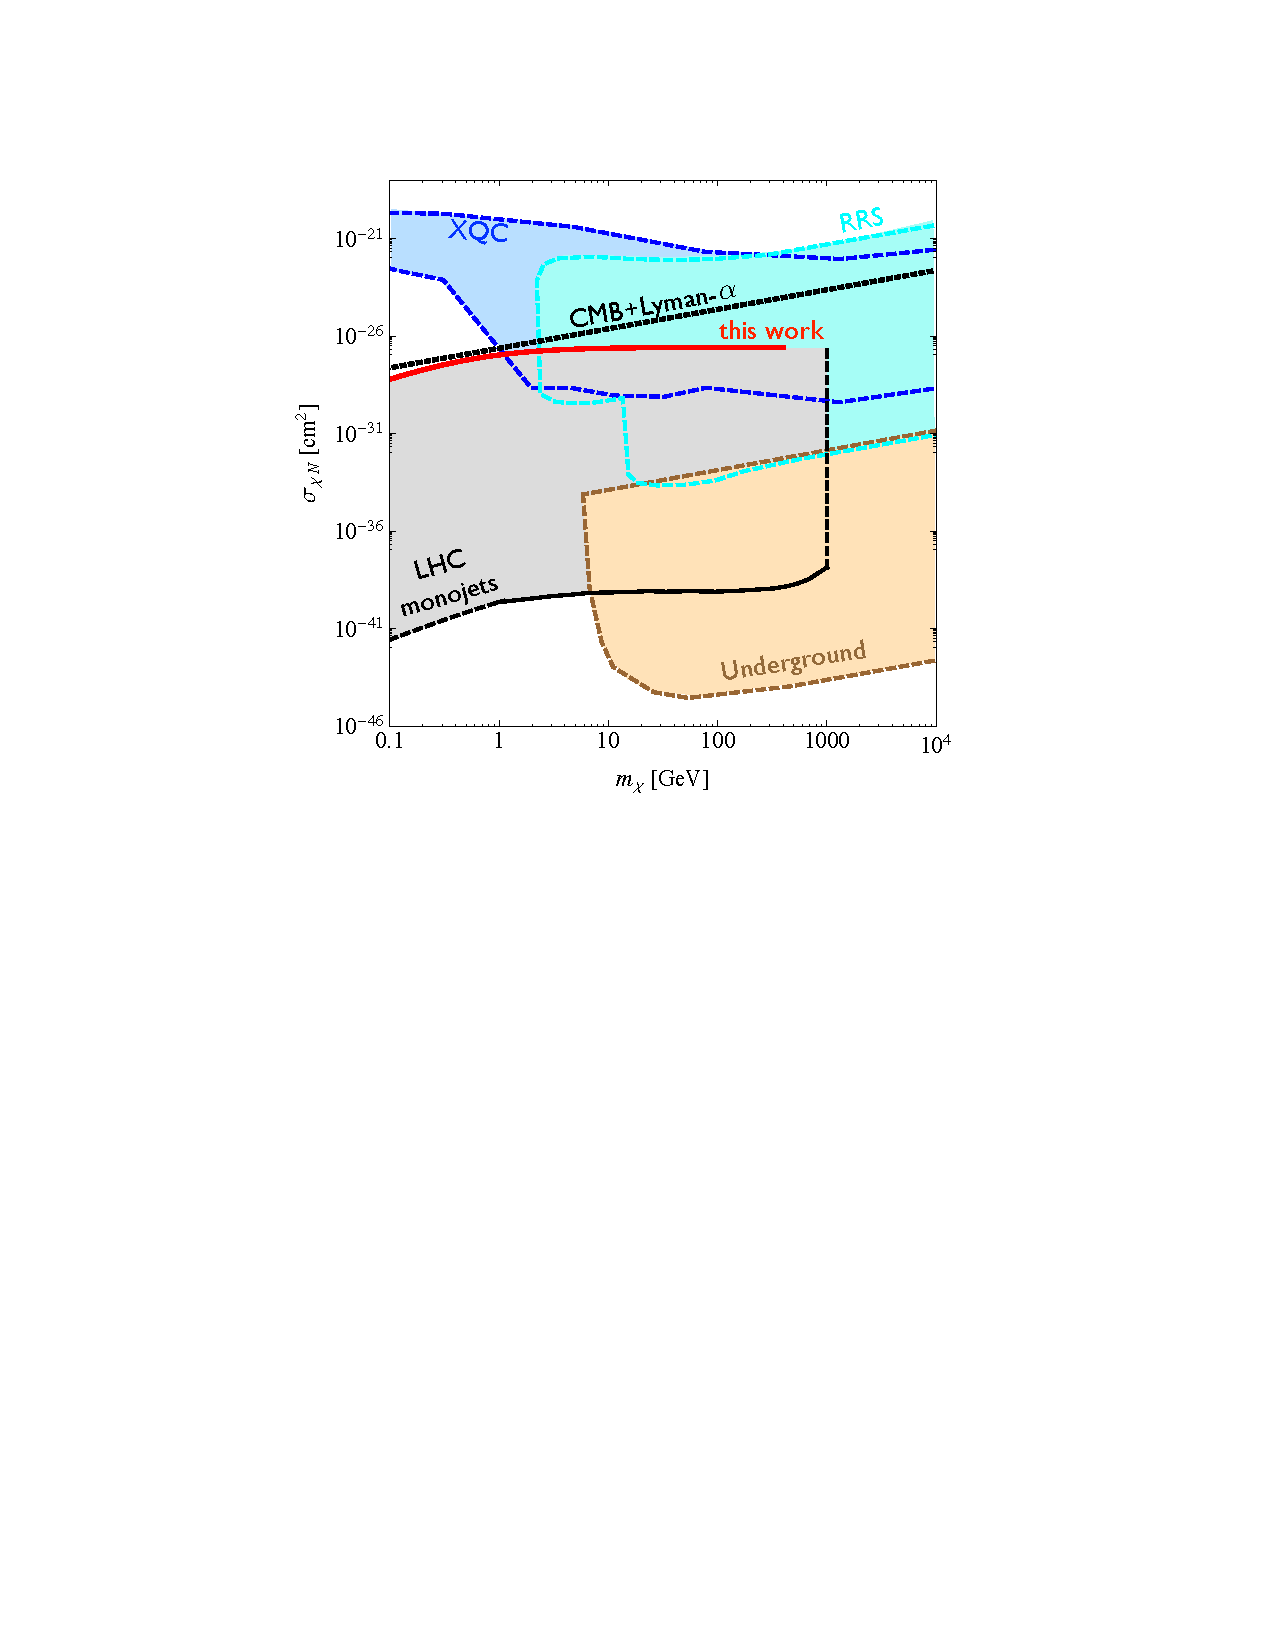
\includegraphics[width=0.5\textwidth]{plots/simps_constraints.pdf}
\caption{Astrophysical and collider constraints on a simple SIMP setup. Note that the relevance of the astrophysical constraints depends on the contribution of the SIMPs to the relic density. Taken from reference~\cite{Daci:2015hca}.}
  \label{fig:simps}.
\end{figure}


\section{Overview of Gaps}
\label{sec:covgaps}

\begin{enumerate}

	\item All-hadronic
	\begin{itemize}
	\item Use associated object triggers (especially motivated by Higgs like VBF and VH)
	\item Try to push to lower masses \& lifetimes
	\item Online reconstruction of hadronic displaced objects
	\item Exclusion limits for displaced hadronic taus. Opportunity for CMS displaced triggers?
	\end{itemize}

\item Leptonic	
	\begin{itemize}
	\item Intermediate region between low-mass (lepton-jets) and high-mass (resolved ATLAS/CMS searches)
	\item Continue to push to go to lower masses, $p_{\rm T}$ thresholds
	\item Tau leptons in LLP decay, in particular if they come from ID. Opportunity for CMS displaced triggers?
	\end{itemize}
	
	\item Semi-Leptonic	
	\begin{itemize}
	\item Low masses (like Majorana neutrino)
	\item Making sure to cover all flavor combinations (for example, one CMS search only covers $e^\pm\mu^\mp$), as well as same-sign vs.~opposite sign leptons
	\item Trigger on associated objects or use dilepton trigger if there are two LLPs?
%	\item 
	\end{itemize}
	

	
\item Photonic
	\begin{itemize}
	\item No coverage for LLPs decaying into $l \gamma$, $j \gamma$ or without $\metm$.
	\item Poor coverage (non-dedicated search) for single $\gamma$, only if two jets are present, needs recasting of CMS delayed photon study~\cite{CMS:2015sjc}.
	\item Prompt photons searches useless, as they veto "non-standard" photons.
	\item No coverage for softer photons.
	\end{itemize}
	
\item Other exotic long-lived signatures
	\begin{itemize}
	\item DTs: $c \tau \sim $ mm are very hard to probe. See suggestion in~\cite{Ito:2017dpm,Ito:2018asa}. Unclear if ATLAS IBL will be present in HL-LHC run. What is the lowest distance new layers (or double layers) can be inserted at? 
%	\item 
	\end{itemize}	

	

\end{enumerate}


%\bibliographystyle{JHEP}
%\bibliography{LLPs}
%
%
%\end{document}
